\documentclass{article}
\usepackage[utf8]{inputenc}
\usepackage[english]{babel}
\usepackage{csquotes}
\usepackage[left=3.5cm,right=3.5cm,top=3cm,bottom=3cm]{geometry}
\usepackage{parskip}
\usepackage{amssymb}
\usepackage{amsmath}
\usepackage{amsthm}
\usepackage{mathtools}
\usepackage{wrapfig}
\usepackage{booktabs}
\usepackage{longtable}
\usepackage[dvipsnames]{xcolor}
\usepackage[skip=2pt,font=small]{caption}
\usepackage{url}
\usepackage{graphicx}
\usepackage{listings}
\usepackage{fancyhdr}
\usepackage{lastpage}
\usepackage{caption}
\usepackage{subcaption}



\pagestyle{fancy}
\fancyhf{}
\lhead{Project}
\rhead{34229 Project Work - Bachelor in Cyber Technology}
\cfoot{Side \thepage{} af \pageref{LastPage}}

\definecolor{codegreen}{rgb}{0,0.6,0}
\definecolor{codeblue}{rgb}{0,0,1}
\definecolor{codegray}{rgb}{0.5,0.5,0.5}
\definecolor{codepurple}{rgb}{0.58,0,0.82}
\definecolor{backcolour}{rgb}{0.95,0.95,0.92}

\lstdefinestyle{mystyle}{
    backgroundcolor=\color{backcolour},   
    commentstyle=\color{codegreen},
    keywordstyle=\color{codeblue},
    numberstyle=\tiny\color{codegray},
    stringstyle=\color{codepurple},
    basicstyle=\ttfamily\footnotesize,
    breakatwhitespace=false,         
    breaklines=true,                 
    captionpos=b,                    
    keepspaces=true,                 
    numbers=left,                    
    numbersep=5pt,                  
    showspaces=false,                
    showstringspaces=false,
    showtabs=false,                  
    tabsize=2
}

\lstset{style=mystyle}
%Biblatex
\usepackage{biblatex}
\addbibresource{Internet.bib}


\begin{document}



\begin{titlepage}

\newcommand{\HRule}{\rule{\linewidth}{0.5mm}}

\center

\textsc{\Large Danmarks Tekniske Universitet}\\[1.5cm]


\includegraphics[scale=0.15]{Billeder/DTULogo.png}\\[1.3cm]

\HRule\\[0.5cm]

{\huge\bfseries WiFi-scanning, Deauthentication and WEP Password cracking}\\[0.4cm]

\HRule\\[1.3cm]

\textsc{\Large Final Report}\\[1.5cm]

\textsc{\Large34229 Project Work\\ Bachelor in Cyber Technology}\\
\textsc{\Large }\\[1.5cm]


\begin{minipage}{0.5\textwidth}
        \begin{flushleft}
            \centering
            \large
            Authors:\\
            Oliver Brisson Bredel (s214684) \\[0.2cm]
            Lucas Loua Buhelt (s214691) \\[0.2cm]
            Nicklas Thorvald Kiær (s216137) \\[0.2cm]
            \hfill \break
            Adviser: 
            \\Henrik Wessing \\[0.2cm]
        \end{flushleft}
\end{minipage}
\\[1cm]
\vfill \vfill

{\large 20. June 2023}

\vfill

\end{titlepage}


\newpage

- Hvor udbredt er sårbarheden
- Mitigation afsnit
- Er client tilsluttet eller er det bare kommu - Oliver - donski (sådan da)
- Sætte angrebene i kontekst med cyber kill chain?
- Løse Kommentarer
- Tests tilføjes mere - done?.
- Implimentation, nye ting ( fx. Json)
- Vi skal have noget med om vores metodik i opgaven, fx det her med at følge PEP8 standard og at vi har lavet agil (?) software development..


\textbf{Hvad er done?
}Abstact - DONE
Contributers - Mangler (sidste ting)
Introduction - DONE
Functionality - DONE
Theory - Mangler kort afsnit om problem ved deauthentication 
Implementation - Figurer osv skal placeres godt, 
Tests - DONE
How to run - DONE
Discussion - Mangler noget om udløbsdato på angrebene, diskussion om resultaterne
Conlusion - Skal genemarbejdes yderligere (må gerne være lidt længere if need be)
Peer feedback - DONE
Collaborative Experience - Kun snakke om tidsplan en gang


\section*{Abstract}
The main goal of this project is to explore and examine the properties of the 802.11 specification. Wireless communication/security is critical to maintaining the internet infrastructure and is widely used, therefore it is a focus of both hackers and network administrators. As data is sent over a shared medium it is possible to both obtain and manipulate it . By doing so, two attacks have been examined in this report. A Denial-of-Service (DoS) attack has been exploited on the wireless local area network (WLAN) - the deauthentication attack, whilst WEP secret key cracking has been used to obtain clear text traffic. WEP was one of the first ways to encrypt wireless data, but has glaring flaws in its algorithm. It's been possible to crack the password for a network secured by WEP and shown that by capturing packets from a single user on an AP, all data that has been sent over the medium can be decrypted. The WLAN has been mapped by with a network interface in monitor mode and data processing using Scapy (Python library) in connection with our deauthentication attacks that show key information on the WLAN. A deauthentication attack has been successfully completed on a modern device after identifying it with the self-developed tool named WiFi-scanner. This shows that even secure networks using technologies in use today, are still at risk of certain attacks.

\newpage
\tableofcontents
\newpage

\section*{Contributers}

\begin{table}[!htbp]
\centering
\begin{tabular}{|l|l|l|}
\hline

\textbf{Section}   & \textbf{Contributer} & \textbf{Reviewer} \\ \hline
Abstract           & Oliver               & Lucas             \\ \hline
Introduction       & Nicklas              & Oliver            \\ \hline
Functionality      & Everyone             & Everyone          \\ \hline
Theory 4.1         & Lucas                & Oliver            \\ \hline
Theory 4.2         & Nicklas              & Oliver            \\ \hline
Implementation 5.1 & Oliver               & Nicklas           \\ \hline
Implementation 5.2 & Nicklas              & Lucas             \\ \hline
Implementation 5.3 & Lucas                & Oliver            \\ \hline
Tests 6.1          & Oliver               & Lucas             \\ \hline
Tests 6.2          & Nicklas              & Lucas             \\ \hline
Tests 6.3          & Lucas                & Nicklas           \\ \hline
Discussion         & Nicklas              & Oliver            \\ \hline
Conclusion         & Nicklas              & Oliver            \\ \hline
\end{tabular}
\end{table}

\section{Introduction}
Wireless security has become increasingly critical due to the rapidly expanding use and need for internet access. Many devices use WiFi to connect to the internet, such as smartphones and laptops. As data over WiFi is sent via radio waves, thus using a shared medium there is a coherent risk when communicating. The data is at risk of being captured by bad actors and is prone to manipulation. Thus a need for strong encryption and control of said data is necessary. However, some security measures for wireless networks, still have vulnerabilities to exploit. One such attack, which is a focus of this report, is a denial-of-service (DoS) attack: the deauthentication attack. It's an attack where a user will be denied access to the network and thereby either disrupt a workplace or pave the way for other more sophisticated attacks such as the Evil Twin Attack\footnote{An Evil Twin attack is when the adversary creates an AP identical to the victim's, and then either forcing or tricking the victim's devices to connect to the malicious AP, thus obtaining a Man-in-the-Middle state.}.

This project will explore the theory and practical applications of deauthentication attacks on networks. Further, password cracking will be explored for secret keys used in the encryption of wireless network traffic using the now outdated WEP protocol. To achieve these goals, information about the wireless local area network (WLAN) has to be known. Thus, another goal for the project is  to obtain information of available SSIDs, clients connected, signal strength and so on.

By doing this project we have explored the theory and practical applications of deauthentication attacks on networks and the building blocks that make up data-packets in a wireless network. By extension of this we have also acquired knowledge about how an access point (AP) connects and disconnects clients and how a local network is built. It is important to note that this project is for educational purposes only and should not be used for malicious activities.


\section{Functionality}
Our project consists of the following functionalities:
\begin{enumerate}
    \item Scan the WLAN and identify key information about clients/Access Points.
    \item Perform deauthentication attack on WiFi devices.
    \item Capture packets and obtain clear text by cracking the password of WEP encryption.
\end{enumerate}

These functionalities represent the core of the project. Wherein scanning and mapping the WLAN, is of a great importance. As this is necessary for performing both deauthentication and password cracking. 

A typical user road-map utilizing the scanning of the network in order to deauthenticate the user is shown on figure \ref{user-roadmap}.  

\begin{figure}[!htbp]
    \centering
    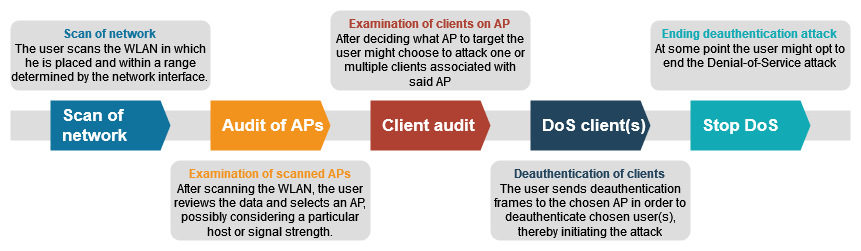
\includegraphics[width=0.9\textwidth]{Latex-Files/Billeder/Flowcharts/user-roadmap.png}
    \caption{A typical user road-map}
    \label{user-roadmap}
\end{figure}

A deauthentication attack is a type of Denial-of-Service (DoS) attack that targets communication between a user and a WiFi access point \cite{Deauth}. It exploits a feature of IEEE 802.11 wireless networks that allows devices to disconnect from a network by the deauthentication management frame \cite{Deauth_Wiki}.
A deauthentication frame tells a device to stop communicating with the AP. It can be sent by either the AP or the device itself. It's normally used for legitimate purposes, such as ending a connection or switching to another network (handover); Yet there is no identification check performed in this procedure. Therefore an attacker can exploit this feature and send deauthentication frames to the AP with a spoofed\footnote{Spoofed: An illegitimate address to trick a victim.} client source address. This causes the connection to close making the spoofed device's connection end and probably reconnect. This exploitation has multiple use-cases. If done repeatedly or to multiple devices, this can disrupt or disable the network entirely, thus resulting in a DoS Attack. Meanwhile it can also be used to obtain an EAPOL 4-way-handshake for WPA or as a way to misguide a client to a rogue access point created by a malicious user to obtain a Man-In-The-Middle state, known as an Evil Twin Attack. 

\begin{figure}[!htbp]
    \centering
    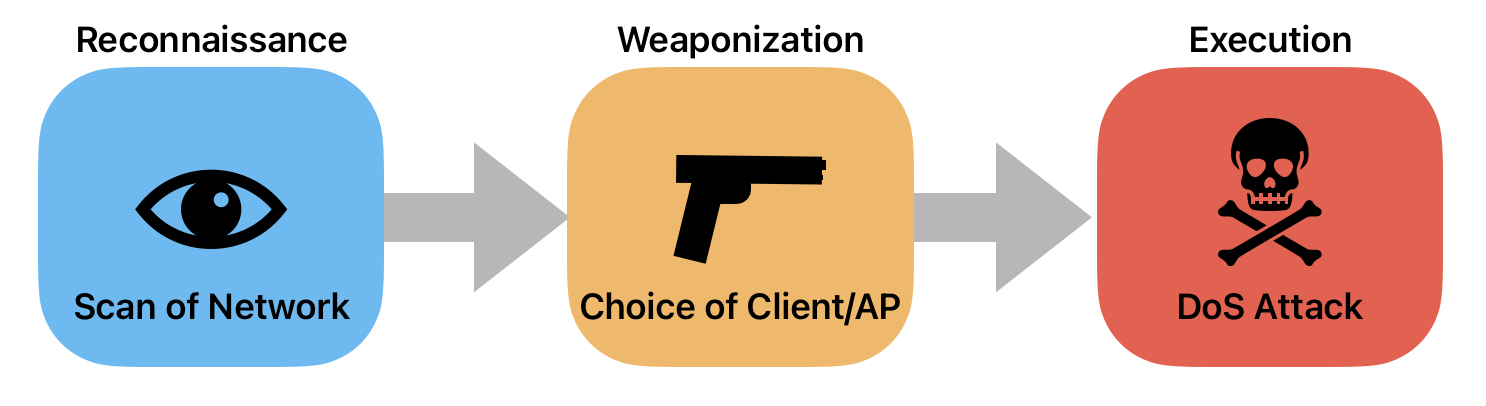
\includegraphics[width=0.5\textwidth]{Latex-Files/Billeder/Lockheed Martin.png}
    \caption{Lockheed Martins's Cyber Kill Chain for our project}
    \label{kill-chain}
\end{figure}


Comparing this attack with Lockheed Martin's Cyber Kill Chain and Mitre's Att\&ck framework the "Scan of network" function would be the reconnaissance of the attack, with the technique T1590 Gather Victim Network Information \cite{lockheed} \cite{Mitre}. Then the two audits (Client and AP) could be signified as Resource Development (Mitre) or Weaponization (Kill Chain) as it is here chosen what clients/AP to spoof. The when the DoS attack happens the Execution/Exploitation happens such that the impact will be DoS and thus the technique T1489  Service Stop.  Hence this is a somewhat simple attack as much of the Mitre Framework is applied, yet it goes through the whole Kill Chain and can thus be a standalone attack, instead of other typical attacks focusing only on reconnaissance or Privilege Escalation.

The last point is password cracking. The product is able to crack a network and obtain the AP's password if that AP uses the WEP algorithm. WEP is one of the most basic WiFi algorithms. It is an outdated and non-secure algorithm and the product utilizes Aircrack-ng's FMS\footnote{A Fluhrer, Mantin and Shamir attack} attack to recreate the passwords on the APs \cite{aircrack-ng}. It is a method wherein you can use initialization vectors (IVs), which are created in the WEP algorithm to recreate the password used to encrypt the data. The method needs data-packets from users on the network containing initialization vectors and those are captured by the WiFi scanner, as that is its primary functionality. It needs about 250.000 packets which it stores in a file that is then read by Aircrack-ng which then cracks the password. 

The implementations are mainly based on the python library Scapy \cite{scapy} to implement the functionalities. As our network interface has to be put in monitor mode a UNIX environment is used. 
The network interface is both a Realtek DWA 131-E1 dongle and the Qualcomm Atheros UB93 dongle. The Realtek dongle is used as it is cheap and allows for the usage of monitor mode and very well models a typical client whereas the Qualcomm dongle is used to signify and model a more sophisticated actor, which typically would use stronger and more technical hardware. Thus a typical setup is with the client using the Realtek dongle and the emulated attacker using the Qualcomm dongle.
The UNIX platform has the consequence of limiting the use of the implementation to a specific platform. Though this should be able to be ported to Windows and MacOS if need be. Here the Linux-sub-system (WSL) on Windows might be exploited \cite{WSL_exploit}.
The positive side of using UNIX is that we can implement the program on many types of systems as we use a virtual machine to create the product and the tool being relatively easier to port to other systems. Thus making a possible conversion to a raspberry pi easier. The negative side is that the use of a virtual machine is mandatory on other operating systems, which can create problems with drivers and performance. 

\subsection{Mapping of networks}
This block takes the physical data being sent in the wireless 2.4 GHz medium, and transforms it into information that the other blocks need and use. It stores a table that holds the information as sub-blocks, for instance access points (AP) in the WLAN, the signal strength of the AP and which channels are used as well as the clients on said AP. This mapping can be done via beacon management frames used by APs to announce their respective presence. Likewise probe management frames can be used to understand what APs a client has been associated with in the past.
Furthermore the block possesses the ability to save the network topology as a png and a json file. This makes it easier to understand the local topology as well as providing the user with the possibility of further analysis using 3rd party software.
The block also contains a way of collecting data-packets containing initialization vectors and sending them to the password cracking block. 


\subsection{Deauthentication}
This block handles the creation and transmission of the deauthentication packets used for the deauthentication attack, it is here the deauthentication packets are spoofed with the desired BSSIDs and then deployed to attack the AP in question. The transmission of the deauthentication packets is tested for optimal performance utilizing the equipment we have had access to. 

\subsection{Password cracking}
This block handles the actual cracking of WEP from data-packets collected from the mapping block. It handles all traffic sent over a specific channel and then filters only for WEP packets. The data is combined into a single file which Aircrack then analyses and gets the password of the AP.

\section{Theory}

\subsection{Network scanning and 802.11}
The primary conceptual framework of this project revolves around the 802.11 standard \cite{IEEE802.11}. The 802.11 standard is a set of wireless network protocols developed by the Institute of Electrical and Electronics Engineers (IEEE). The first version of the standard, 802.11, was released in 1997, and since then, several revisions and amendments have been made to improve the technology and increase its capabilities \cite{ETHW}.

The 802.11 standard uses radio waves to transmit data between devices within a WLAN without the need for cables or wires. This makes it a popular choice for connecting mobile devices to the internet, especially in homes, offices, and public places such as cafes, airports, and hotels \cite{Public_WiFi}.

\begin{figure}[!htbp]
    \centering
    \includegraphics[width=0.5\textwidth]{Latex-Files/Billeder/WiFi_Types.png}
    \caption{WiFi types and Subtypes, \cite{frame_types}}
    \label{WiFi Types}
\end{figure}

There are three frame types in 802.11: management frames, control frames, and data frames.\cite{Amit802.11frames, DefinitiveGast}. Figure \ref{WiFi Types} shows some of the types and subtypes of different frames with a focus on management frames, since that is what our project is focused on.  Management frames are used by APs to join and leave the basic service set (BSS). They have a MAC header, a frame body, and a trailer. These frames are needed do to the difficulty of connecting to a wireless network compared to a wired network. With a wireless connection, all data is sent everywhere and each router and user needs to know which data-packets to ignore and which to receive. This is done via management frames where a user associates with an Access Point (AP) and agree on conditions, such as security and speed. For a user to know which APs are near, it needs to scan the surrounding area. 

This is done via 2 ways of scanning: Active scanning and passive scanning. 
As an 802.11 environment is an open medium, the packets sent over the network are easily obtained by bystanders. Yet the amount of traffic sent is governed by the clients and APs. Thus enabling passive scanning to obtain data frames sent over the medium with no involvement. Active scanning is different in the way that it also obtains the packages the same way, but here the scanner actively joins the communication in the hope of stimulating the clients/APs/targets to provide/send more data \cite{Mitre2}.
The amount of data sent is often non-deterministic, since a client, in principle, can be connected to an AP without sending any information or data for long periods. Therefore making determining the relation between a client and an AP challenging. Yet it is normal for clients to send out probe requests and in general a modern client sends more data. A paper from 2014 shows that background traffic constitutes 40\% of traffic \cite{utility}. With mobile devices accounting for over 50\% of all traffic, there is a lot of data sent even without the user actively using the device \cite{stats_mobile}.
However it is easier to estimate the amount of beacon frames sent from an AP, which is one of the most obvious frames to scan for. As beacon frames contains a field called Beacon interval containing the time interval between each beacon frame in Time Units (1024 microseconds). This can be used to understand how long one should scan in a given channel in order to be sure that a beacon frame has been obtained.
Since at least one beacon frame is needed and it has to be obtained in full it can be argued that a period of at least two beacon intervals has to be observed in each channel. Therefore the time in each channel is given by:
\begin{align}
    t_{channel} >= 2\cdot beacon_{interval}
    \label{tchannel}
\end{align}
Thus the overall time to scan for APs will be:
\begin{align}
    t_{all\_channels} = t_{channel}\cdot number_{channels}
    \label{tallchannels}
\end{align}
Where the number of channels most often is 14 and the beacon interval 100TU.

\subsection{The Scapy library}
This project utilizes the python library "Scapy" for sniffing, analyzing and transmitting 802.11 packets. Scapy is a complex and substantial program and library built in Python with a plethora of functionality. One example of functionality Scapy, used for this project is the "sniff" function. This enables users to capture network packets sent on the wireless medium. 
The packets captured are described as Scapy packet objects. Wherein Scapy internally decodes captured packets, and defines the packet object with layers corresponding to the protocol layers used the packet. The packet object consequently contains a great amount of information about the packet. This information includes SSIDs, BSSIDs, channels, cryptographies and more. 
Scapy can furthermore be used to create and send packets via the same methods as decoding these packets. 

\begin{figure}[!htbp]
    \centering
    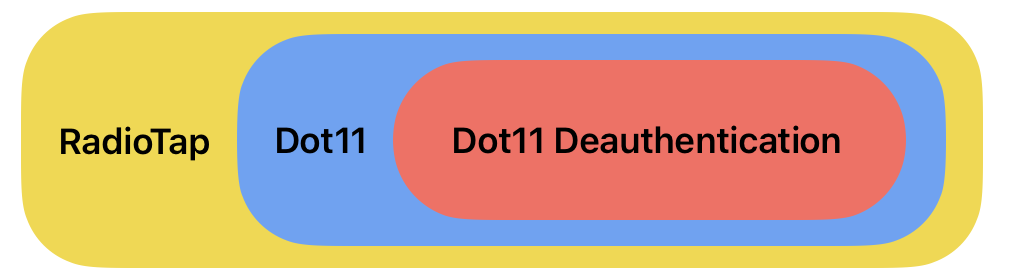
\includegraphics[width=0.5\textwidth]{Latex-Files/Billeder/scapy_packet.png}
    \caption{Scapy deauthentication packet illustration}
    \label{scapy_packet}
\end{figure}

An example of the creation of a packet can be seen in figure \ref{scapy_packet}. Wherein a deauthentication packet is built, by stacking layers on top of each other. For the deauthentication packet, the Radiotap layer serves as the foundation of the packet. The Radiotap layer contains properties such as signal strength, channel information etc. This is followed by a "Dot11" layer on top, this layer describes, among other things, the type and subtype of the packet, in this case "type = 0" which represents a management frame and "subtype = 12" which represents a deauthentication packet. Ultimately the "Dot11Deauth" layer is added, this layer provides the ability to alter the reason code sent with the deauthentication packet, indicating the reason for the deauthentication.\cite{Scapy_documentation}


\subsection{Deauthentication in WLAN}
The connection between clients and APs can be exploited by deauthentication attacks. The theory behind this attack is based on the 802.11 standard, which allows clients to disconnect from an AP using a deauthentication frame\cite{IEEE802.11}.

\begin{figure}[!htbp]
    \centering
    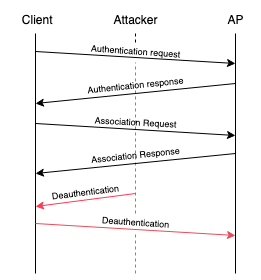
\includegraphics[width=0.3\textwidth]{Latex-Files/Billeder/Implementation/deauth_transmission.png}
    \caption{Flow of Deauthentication attack}
    \label{deauth_flow}
\end{figure}

Figure \ref{deauth_flow} illustrates a deauthentication attack in action, wherein a stable connection is established, but followed by the attacker transmitting a deauthentication packet to the AP, spoofed as the client. Following this the AP sends a deauthentication to the client, thus terminating the connection.

Deauthentication frames are of the management frame type as seen in figure \ref{WiFi Types}, and have the overall structure as such. Therefore the deauthentication frame contains, among other things, three addresses. These addresses being the destination address, the source address, and the BSSID of the AP's wirelsess interface (the two last addresses are often identical). These three addresses are what can be altered in order to spoof packets, and perform a deauthentication attack. One of the fields in a deauthentication frame is the reason code, which is a 16-bit field, thus giving 65,536 unique possible reason codes, yet only about 66 are utilized \cite{Cisco_Deathentication_reasoncodes}. The reasoncode defines the reason for the termination of the connection. Apart from a reason code, the frame body includes vendor specific elements, and the Management MIC IE (MMIE) \cite{IEEE_802.11w}. Though this is only present when protected management frames(PMF) are enabled, further examination of PMF will follow in subsequent sections the report.

Spoofing a deauthentication frame involves forging and sending a deauthentication frame to a target device, falsely claiming to be a legitimate access point or router. This act of deception creates a significant vulnerability within wireless networks, primarily in the form of denial of service (DoS) attacks. The spoofing of packets is possible using Scapy. Where the source address of the deauthentication packet can be spoofed to appear as if the sender is a legitimate AP.
These spoofed deauthentication packets can be sent, thus denying service for clients on the attacked AP.

\subsection{WEP \& WiFi security standards}
Wireless networks also need security while sending packets, i.e. integrity and confidentiality. To ensure confidentiality, data-frames are encrypted with a security standard. The oldest widespread type being Wired Equivalent Privacy (WEP). It had major security flaws that allowed hackers to bypass the algorithm and read the data being sent\cite{WEP1}. Therefore a new protocol for network security was in need. WiFi Protected Access (WPA) was soon after developed and implemented from 2003\cite{WEP3}. 

WEP uses a secret key to encrypt packets sent between a client and the AP \cite{WEP2}. Although, a fundamental underlying problem with WEP is that WEP uses the RC4 encryption algorithm, which is known as a stream cipher. A stream cipher operates by making a short key into a random key-stream. The client uses the XOR operator on the key-stream with the plain data to produce the encrypted data. The AP has a copy of the same used key, and uses it to generate an identical key-stream. The AP then performs the XOR operation on the key-stream with the encrypted data thus obtaining the exact same plain data back. This type of encryption can be decrypted relatively easily. A Fluhrer, Mantin and Shamir attack (FMS attack) uses the initialization vectors (IVs) used in RC4 to crack the WEP algorithm. It needs a certain amount of packets to use statistical analysis to recreate the password uses to encrypt the data.

\begin{figure}[!htbp]
    \centering
    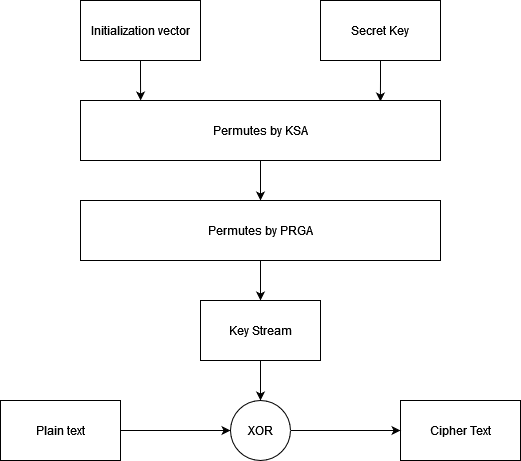
\includegraphics[width=0.4\textwidth]{Latex-Files/Billeder/RC4.png}
    \caption{Simplified RC4 algorithm \cite{geeks}}
    \label{RC4}
\end{figure}

This is because the initialization vector is only a 24 bit field which guarantees the reuse of key-streams because the vector is only made up 24 bits and when thousands or millions of data-packets are sent, reuse will happen often. It would take around 110.000 data-packets to ensure reuse \cite{Random_map}. Because of this, the attacker can easily pick up enough data to perform statistical analysis of packets using the same key-stream and then recover the plain data.

Fortunately mitigation for the flaws of WEP have become industry standard since the WPA2 protocol, which was a development of the intermediate measure WPA as a security update to fix many of WEP's problems \cite{WPA2_1}\cite{WEP3}. It was released in 2004 in the 802.11i amendment to the original 802.11. WPA2 uses CCMP protocol which is a development of the AES security algorithm. It rids the network encryption of the previously mentioned security vulnerabilities. 


\subsection{Mitigation, and vulnerability}
Attacks such as deauthentication and WEP cracking have been around for a long time, and while they still work in some instances, measures have been made in order to mitigate and lessen the effects of such attacks.
\subsubsection{Mitigation of deauthentication attacks}
The deauthentication attacks rely on the possibility of any user to send a deauthentication packet to an AP, wherein the integrity of the deauthentication can be forged. This is possible with deauthentication packets made in cleartext and with no integrity check. In order to mitigate this attack, 802.11w, released in 2009, introduced protected management frames (PMF). These mitigated deauthentication attacks by ensuring the integrity in the management frame. The integrity check is achieved by the sender calculating a Message Integrity Check (MIC) value, and appending this to the frame. The receiver then calculates the MIC value using the same algorithm, and compares the two. If the two MIC values match, the frame is considered to not having been tampered with, thus marking it as authentic. Furthermore a frame sequence number(FSN) is introduced, which is used to prevent replay attacks. \cite{IEEE_802.11w}
Thus mitigation of deauthentication attacks has been achieved when using protected management frames. 

An additional method of mitigating a deauthentication attack, is simply to survey the packets that are being transmitted on the medium. Since the deauthentication attack consists of transmitting deauthentication packets constantly, this can fairly easily be discovered if surveillance of packets being received is possible. For example, our implementation of the deauthentication transmits a deauthentication packet once every 0.005 seconds which is very much noticeable if one was to see the transmitted packets. Therefore by surveilling the medium with a WIDS (wireless-intrusion-detection-system), the deauthentication attack could be discovered.

\subsubsection{Vulnerability of deauthentication attacks}
Though PMF introduced a method of mitigating deauthentication attacks, the use of PMF is still not as widespread as one would think. Since PMF is a setting that should be enabled by the user manually, this is often not done. Thus creating a sizeable vulnerability for many users. The use of PMF will continue to increase in connection with the widening use of WPA3, since PMF are required for WPA3, thus further lowering the vulnerability of deauthentication attacks \cite{WPA3_info}\cite{wpa/pmf}. 

As the system depends on the availability of data frames in order to act and exploit these the system has to be able to obtain these frames. The obvious way is thus to be physically present at the location, consequently doing a so called "on-premise" attack. This has drawbacks as the attacker has to be close to the victim and thus exposing herself to the environment and being easier to catch. Because of this it makes sense to test the equipment's, here the wireless network cards, properties such as how far away from a given victim one needs to be in order to firstly perform the passive scan and secondly perform the required attack (deauthentication or WEP cracking). Similar it can make sense to explore the possibility of creating mobile devices that can be hidden in proximity to the victim, this will be further elaborated at future work. 

\subsubsection{Vulnerability of WEP cracking}
The main vulnerability of WEP cracking is the fact that WEP is not in use today. The widespread adoption of WPA2 and later security algorithms means that WEP cracking is not really a problem today. All cracking of WiFi traffic requires the capture of packets that are being sent. Therefore the best way to stop this would be to make sure that as little sensitive information as possible is being sent over WiFi. The attacker also has to be close to the sender and receiver to collect these packet being sent and so APs could be set to only broadcast in a small area at for example a workplace so that packets can't be collected from outside. 
\section{Implementation}

\subsection{Method}
PEP8 standard, Agil software development, Code-review, 



The implementation is based purely on Python3 and the library Scapy. Figure \ref{UML_diagram} shows a UML-class-diagram of the two classes utilized in the implementation (without CLI and utilization files). The Scanner class can hold multiple WiFi objects. The Scanner class can be seen as the main class holding and performing the core functionalities. Whereas the WiFis are the individual APs that are detected from the network scan, and subsequently saves to the topology.
\begin{figure}[!htbp]
    \centering
    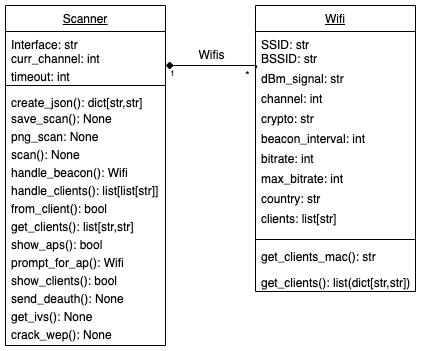
\includegraphics[width=0.5\textwidth]{Latex-Files/Billeder/Flowcharts/classes.png}
    \caption{UML diagram of Scanner and WiFi classes}
    \label{UML_diagram}
\end{figure}
\subsection{Mapping of networks}
The WiFi-scanner is the backbone of our implementation. It listens to all data that is transferred over WiFi and subsequently creates the lists that the deauthentication uses and captures packets for the password cracker. The point of this functionality is to gather information about APs and the associated clients, the logic for this implementation is shown in figure \ref{Flowchart} as a flowchart.

\newpage

\begin{figure}[!htbp]
    \centering
    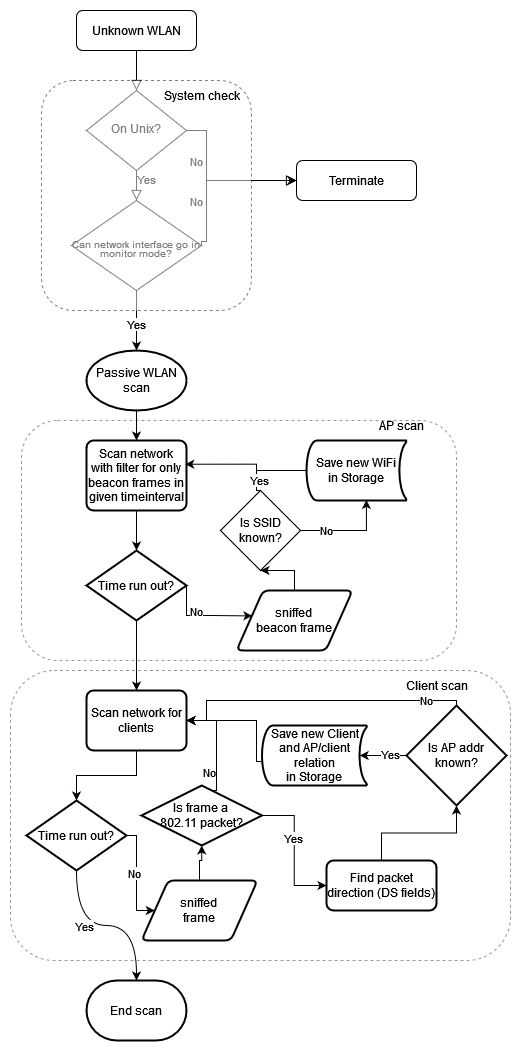
\includegraphics[width=0.8\textwidth]{Latex-Files/Billeder/Flowcharts/network_flowchart.png}
    \caption{Flowchart for mapping of WLAN}
    \label{Flowchart}
\end{figure}

\newpage

Firstly a system check is performed to ensure that the program is running on a UNIX system, as the program is not compatible with other systems. A possible operating system error is shown on figure \ref{W_error}.

\begin{figure}[!htbp]
    \centering
    
\includegraphics[width=0.8\textwidth]{Latex-Files/Billeder/Implementation/Windows_error.png}
    \caption{Windows error}
    \label{W_error}
\end{figure}

Then the program checks if the user is running the program as root, as this is required for Scapy to capture packets and go into monitor mode (this could also be done by creating a special user with the needed groups). The passive scan is split into two main tasks, the first being the scanning for APs and the second being the scanning for clients. 
Even tough it is viewed as two different tasks, the data obtained for the above classification is done once and then processed.
The scanning for APs is done by sniffing for beacon frames, which are sent by APs to announce their presence.

The sniffing is done by using the Scapy function "sniff", which is very similar to wiresharks capture and takes a filter as an argument, this function is used when scanning for APs. The function is set to run for a specified timeout duration. This is done to ensure that the program does not run indefinitely, and thereby potentially causing issues with the system. The code for part of this is shown in figure \ref{Scan1}.
\begin{figure}[!htbp]
    \centering
    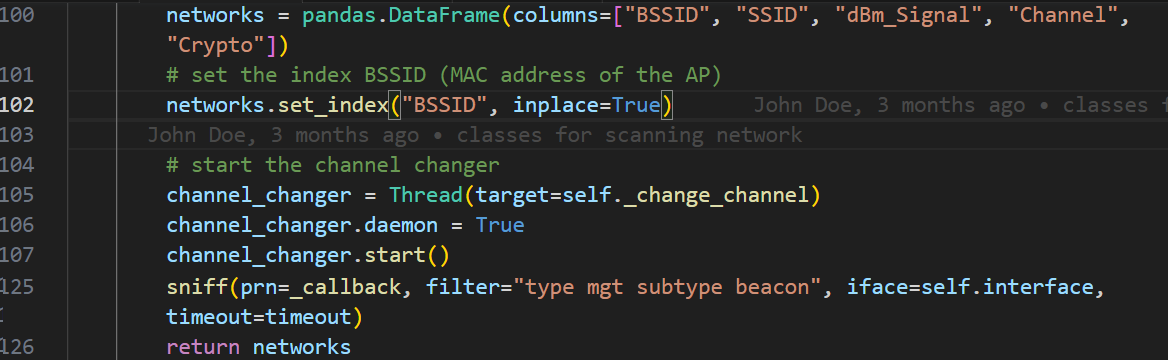
\includegraphics[width=0.6\textwidth]{Latex-Files/Billeder/Implementation/AP_Scan.png}
    \caption{Code for the sniffing with Scapy}
    \label{Scan1}
\end{figure}

The scanning is done on each network channel in turn, where it scans for beacon frames from the APs. It returns the BSSID (MAC-address), SSID, signal strength, channel and the cryptography of each AP and other fields if they exists (country, max bitrate and beacon interval). As the main focus for the scanning is to obtain APs, the minimal time to scan for each channel is found as described in the theory, equation \ref{tallchannels}. Thus by using the general default value of beacon interval at 100 TU and 14 channels the optimal time per channel is 0.205 s and time for the full scan is then 2.87 s.  

This is however a very theoretical value and does not take the time it takes to switch channel into account. Thus examining the time for a scan of all channels gives us approximately 6.11 seconds, thus rounding to 7 makes sure that there is a small wiggle room. This is further shown in figure \ref{timne_to_scan}. Yet it is surprising that the changing of channels is just as time consuming as being in the scan. Further an issue with going through each channel means that some of the 2.4 GHz spectrum is not scanned at all times, thus traffic will be missed. Different approaches to solving this can be done, such as using more interfaces or staying in channels that are more centered thus catching the surrounding channel's traffic as well (such as channel 4 and 8). Yet it has not been deemed important for this project as single data frames are not necessary to create a topology. 

\begin{figure}[!htbp]
    \centering
    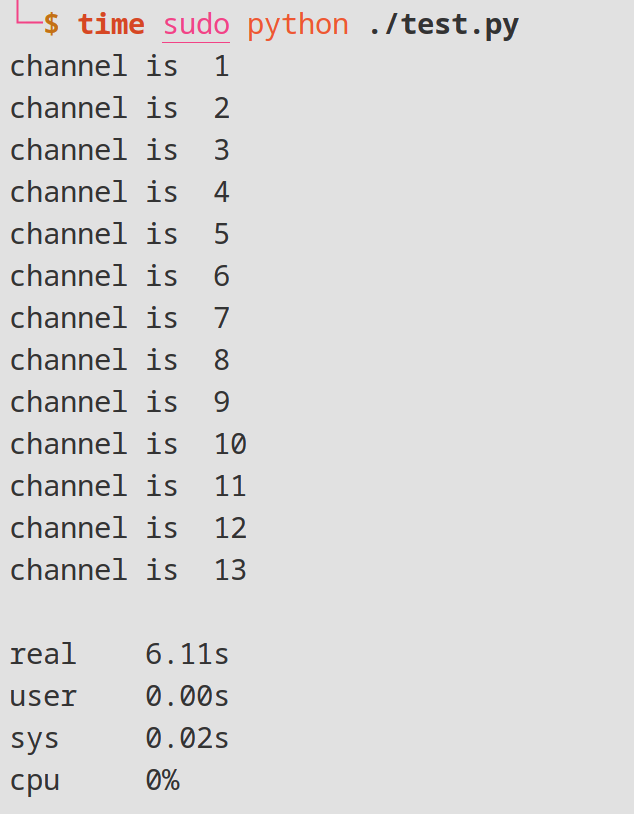
\includegraphics[width=0.45\textwidth]{Latex-Files/Billeder/Implementation/time_to_scan.png}
    \caption{Time it takes to scan all channels}
    \label{timne_to_scan}
\end{figure}
 
When scanning for clients, all 802.11 packets are examined as it is rare that there is communication between APs. However the DS fields in the 802.11 header is exploited, as they indicate the direction of the frame and thus whether it is from a client or not. Discouragingly it can be very hard to classify whether a device is a "true" client to an AP i.e. associated with the AP, as clients often send probe requests to all APs visible. A possible way to resolve this issue is to only use data frames sent between client/AP as the classification feature. Yet as mentioned in the theory section, data sent between client/AP can vary greatly. As we aim to keep the scan time short and the main priority is to obtain information about APs, all data from a device to an AP will make the device classified as a client.  

We use the obtained data that we found and then look at packets being sent and check if the packet is sent from a client. This is then returned with the code shown in figures \ref{get_client1} and \ref{get_client2}. We can see that \lstinline{get_clients()} is the code that gets the clients for each AP.

\begin{figure}[H]
     \centering
     \begin{subfigure}{0.49\textwidth}
         \centering
         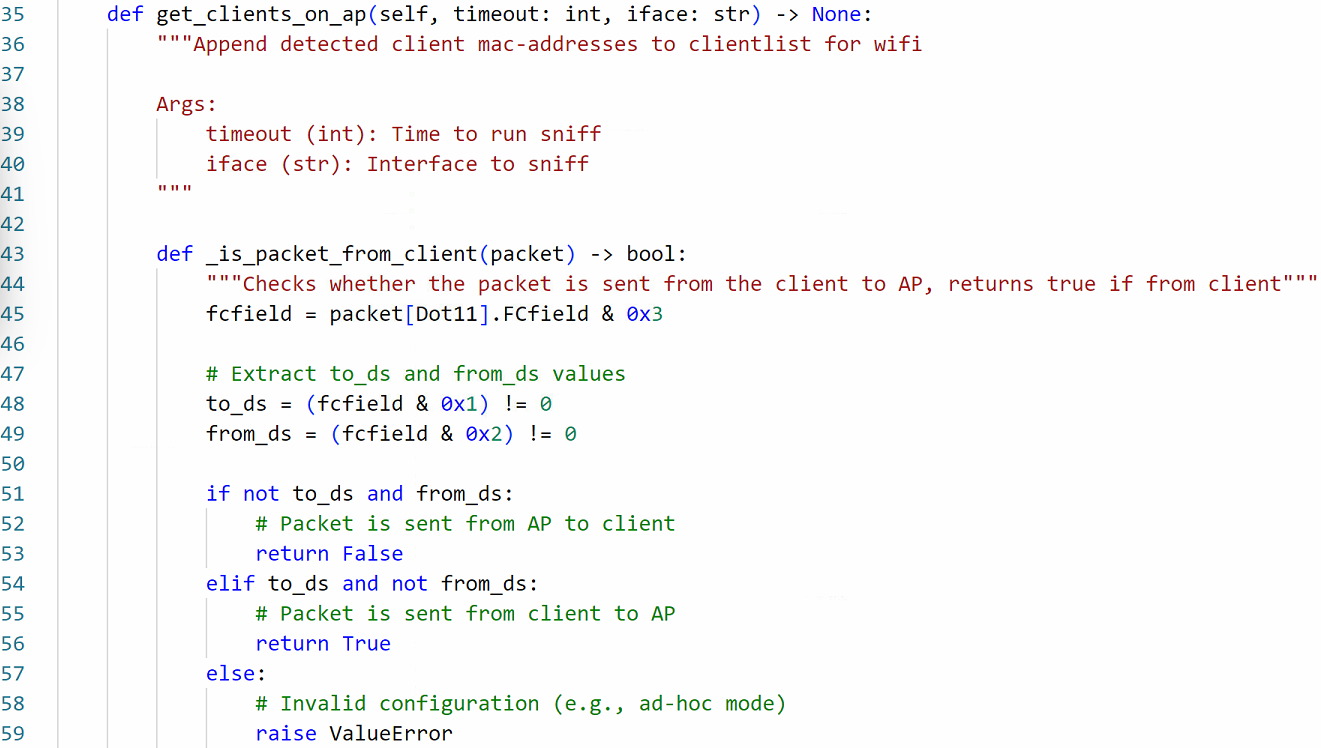
\includegraphics[width=\textwidth]{Latex-Files/Billeder/Implementation/get_client1.png}
         \caption{First part of code for getting client on APs}
         \label{get_client1}
     \end{subfigure}
     \hfill
     \begin{subfigure}{0.49\textwidth}
         \centering
         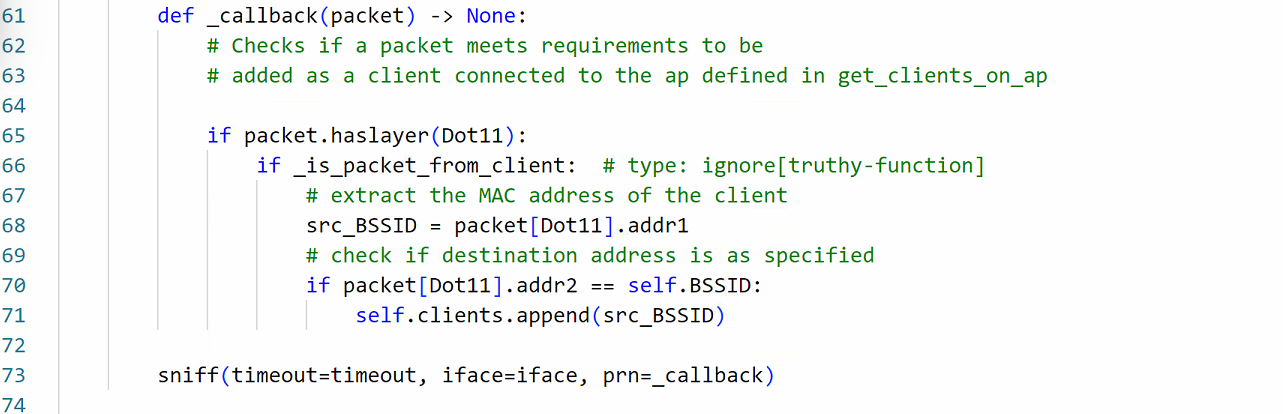
\includegraphics[width=\textwidth]{Latex-Files/Billeder/Implementation/get_client2.png}
         \caption{Second part of code for getting client on APs}
         \label{get_client2}
     \end{subfigure}
     \hfill
     \caption{}
\end{figure}



Further optimization can be done to create better filters and most importantly use all data sent over the medium to create a more complete map of the WLAN. This however has not been done in the current level of implementation and might be deemed unnecessary as the needed data is obtained.

As this tool can be a standalone tool, but could be used in other projects a JSON object of the topology has been implemented based on the WLAN scan. The code for the implementation can be seen on figure \ref{create_json_code}. A scan's JSON object can be seen on figure \ref{json_scan}.

\begin{figure}[!htbp]
    \centering
     \begin{subfigure}{0.49\textwidth}
         \centering
         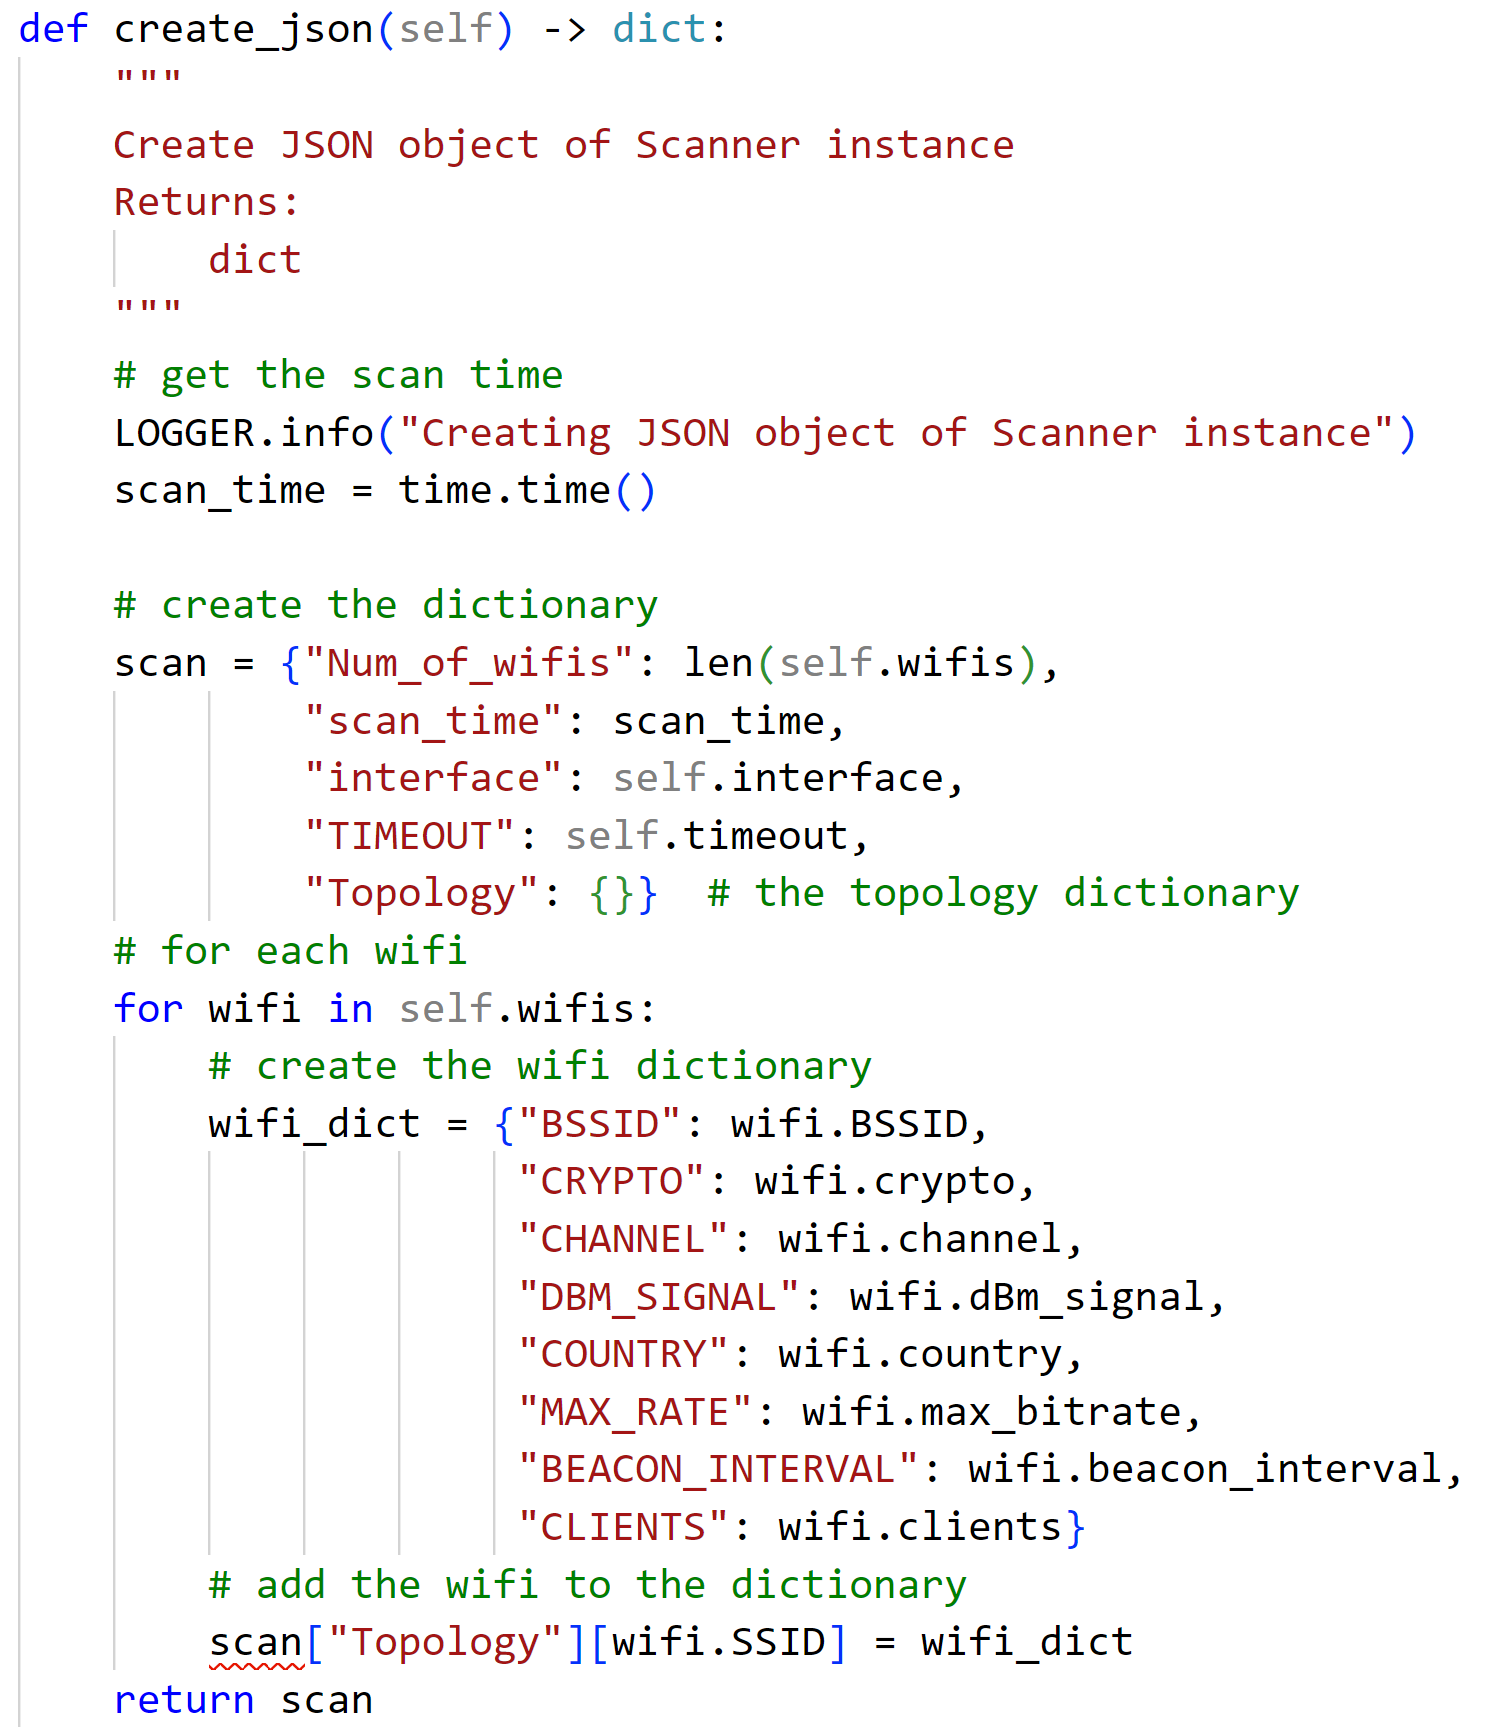
\includegraphics[width=\textwidth]{Latex-Files/Billeder/create_json_code.png}
         \caption{Implementation of json objects based on network scan}
         \label{create_json_code}
     \end{subfigure}
      \begin{subfigure}{0.49\textwidth}
         \centering
         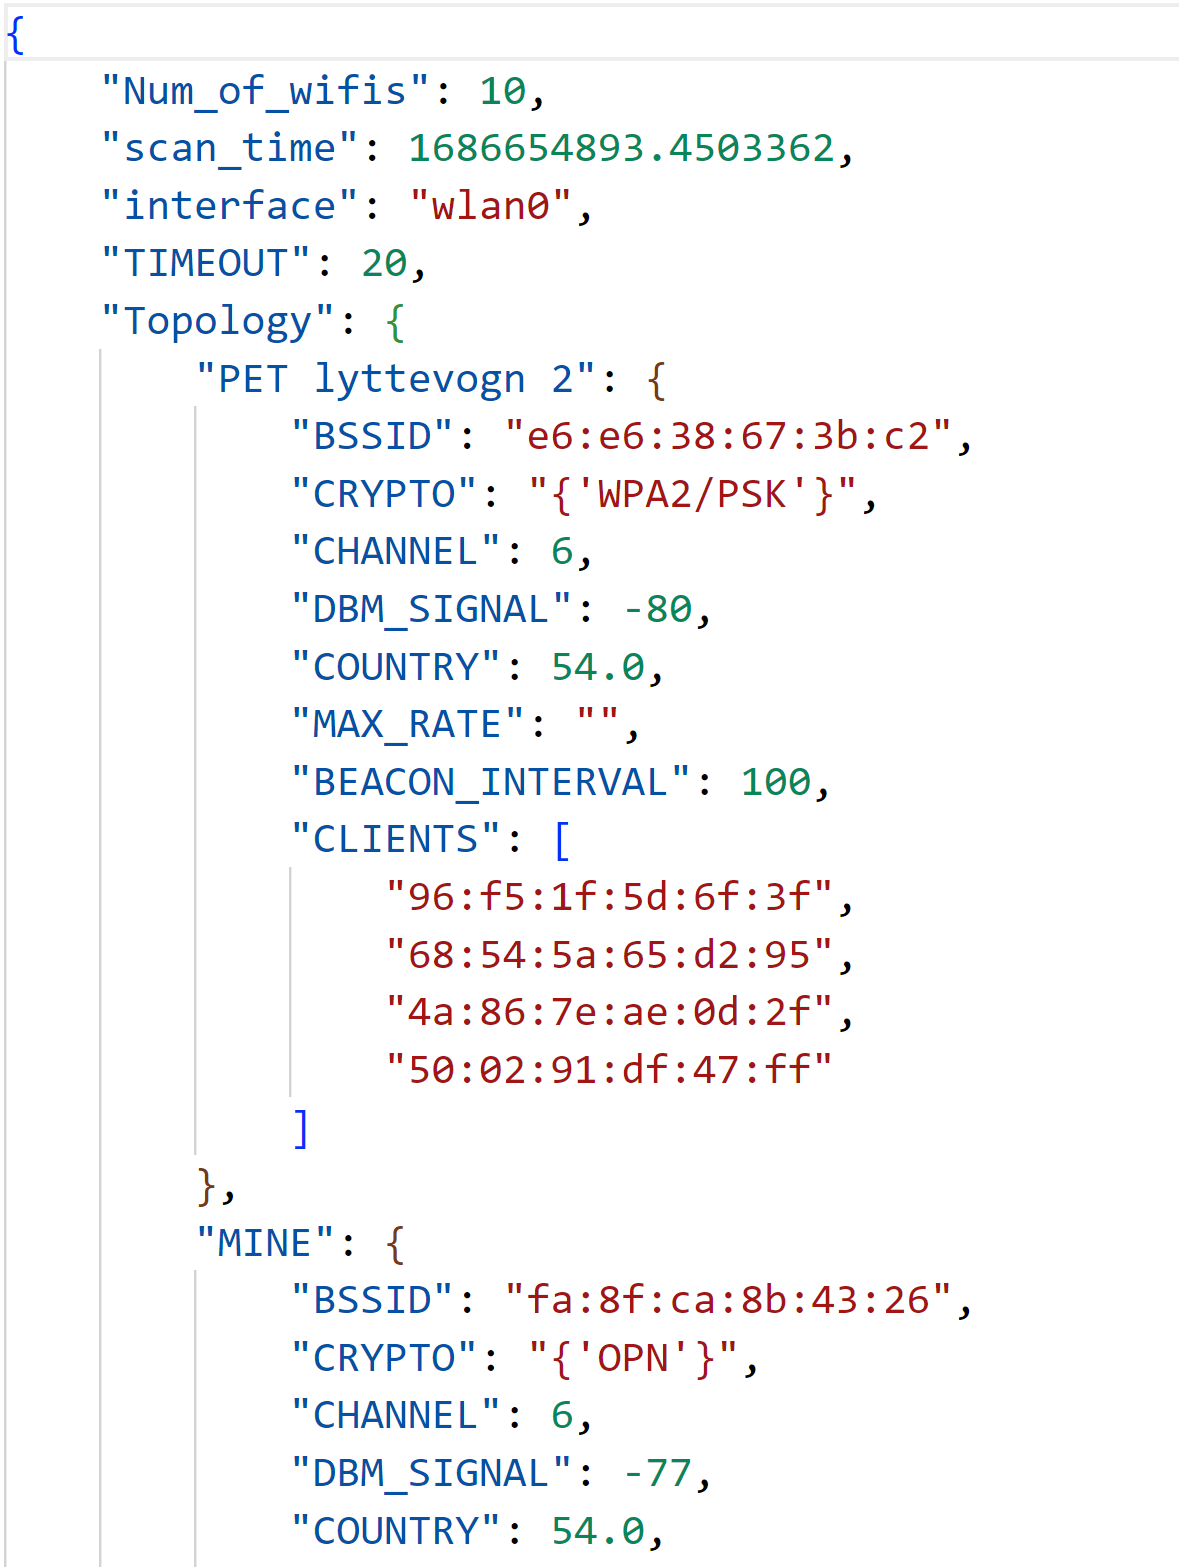
\includegraphics[width=\textwidth]{Latex-Files/Billeder/JSON_object.png}
         \caption{JSON object from scan}
         \label{json_scan}
     \end{subfigure}
     \caption{}
\end{figure}

The topology of the WLAN based on the JSON data from the scan has been used to create a graphical topology for the user. This has been done using the python library networkx. An example can bee seen on figure \ref{network_topology}.

\begin{figure}[!htbp]
    \centering
    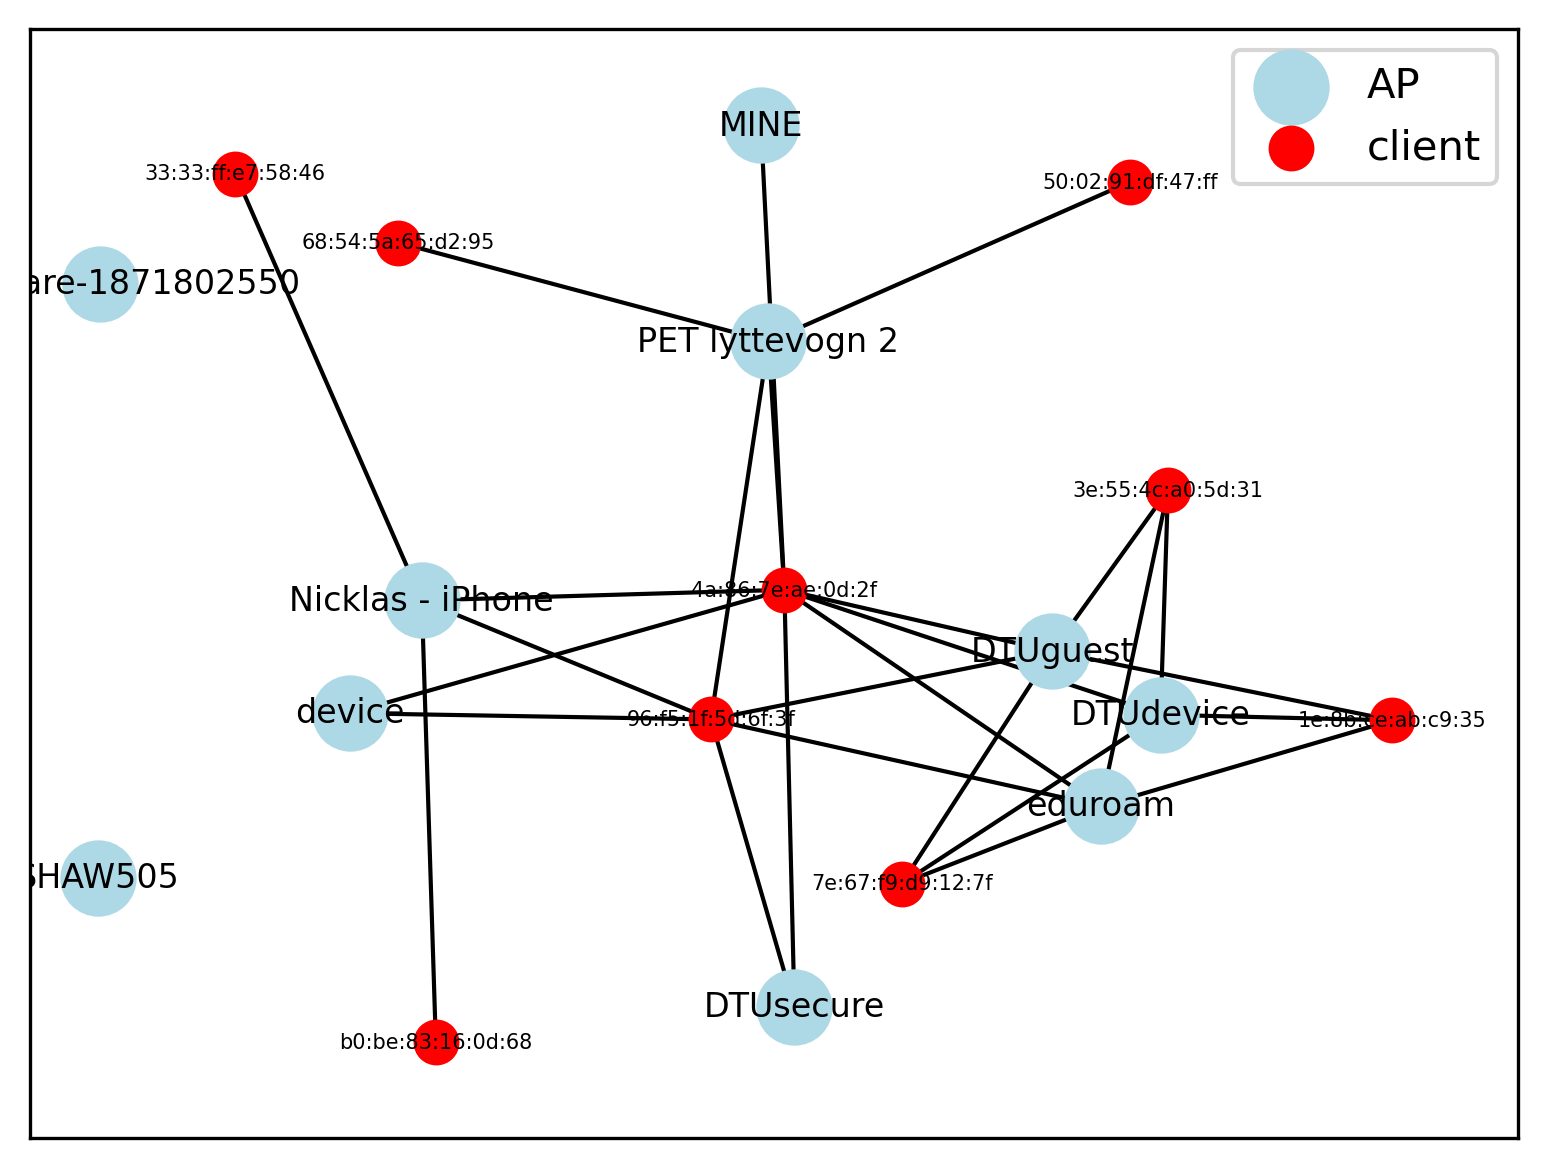
\includegraphics[width=0.5\textwidth]{Latex-Files/Billeder/network_topology.png}
    \caption{Example of a network topology when scanning}
    \label{network_topology}
\end{figure}




\subsubsection{Limitations}
The implementation is limited to only being able to scan for APs and clients in the 2.4 GHz band. This is a physical limitation due to the fact that the dongle used for the implementation only supports the 2.4 GHz band.
The mapping of the network is done by passively scanning the medium, thus resulting in the implementation being limited to only having the ability to scan for APs and clients that are actively sending data. This is a limitation that is inherent to passive scanning. It can be overcome by using active scanning e.g. via a Replay Attack (which can force a device to send specific packets).

When doing the deauthentication attack there is actually a form of active scanning as the system is sending packets to the AP. This is however not a reliable way of scanning for APs and clients, as the current implementation of the attack is not built for this purpose and rather builds upon the passive scanning.

But the limitation of using passive scanning is also one of its positives: Since there is no active participation in the communication, the implementation of the mapping of the network is close to impossible to be detected by a WIDS (WiFi Intrusion Detection System). This is positive as it allows for the implementation to be used for reconnaissance without being detected, whereas active scanning is noisy. For an example there is NMAP: A known tool for mapping networks (on ethernet) that is very noisy and easy to detect.

\newpage
\subsection{Deauthentication}
Our implementation of the deauthentication functionality relies on the ability to create and send packets with the use of Scapy. Thereby forging our own deauthentication packet, thus gaining the ability to set our own parameters for the packet.

\begin{figure}[!htbp]
  \centering
   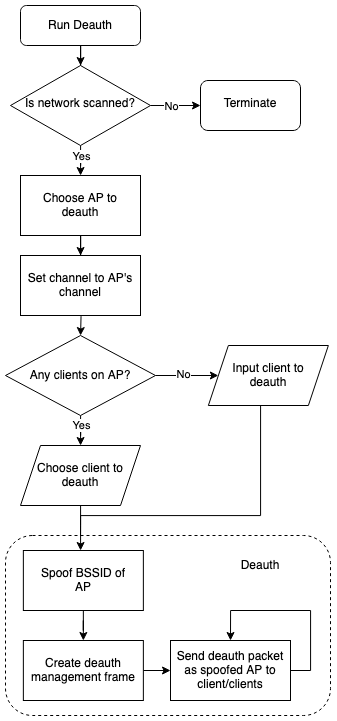
\includegraphics[width=0.5\textwidth]{Latex-Files/Billeder/Flowcharts/deauth_flowchart.png}
   \caption{Flowchart of deauthentication (deauth).}
   \label{flowchart_deauth}
\end{figure}

As shown in figure \ref{flowchart_deauth}, our implementation of the deauthentication is as follows. The implementation in code can be seen in figure \ref{deauth_prompt_code}.

The user is first met with a menu of the known APs, gained from the mapping of the network, that are eligible for attempting an attack.
We have then decided to show another prompt menu which gives the user the option of choosing the target from a list of the already known clients, if so desired. If not, the user can either input a MAC-address, or choose to use the broadcast address, resulting in all clients receiving the deauthentication packets. 

\begin{figure}[!htbp]
     \centering
     \begin{subfigure}{0.49\textwidth}
         \centering
         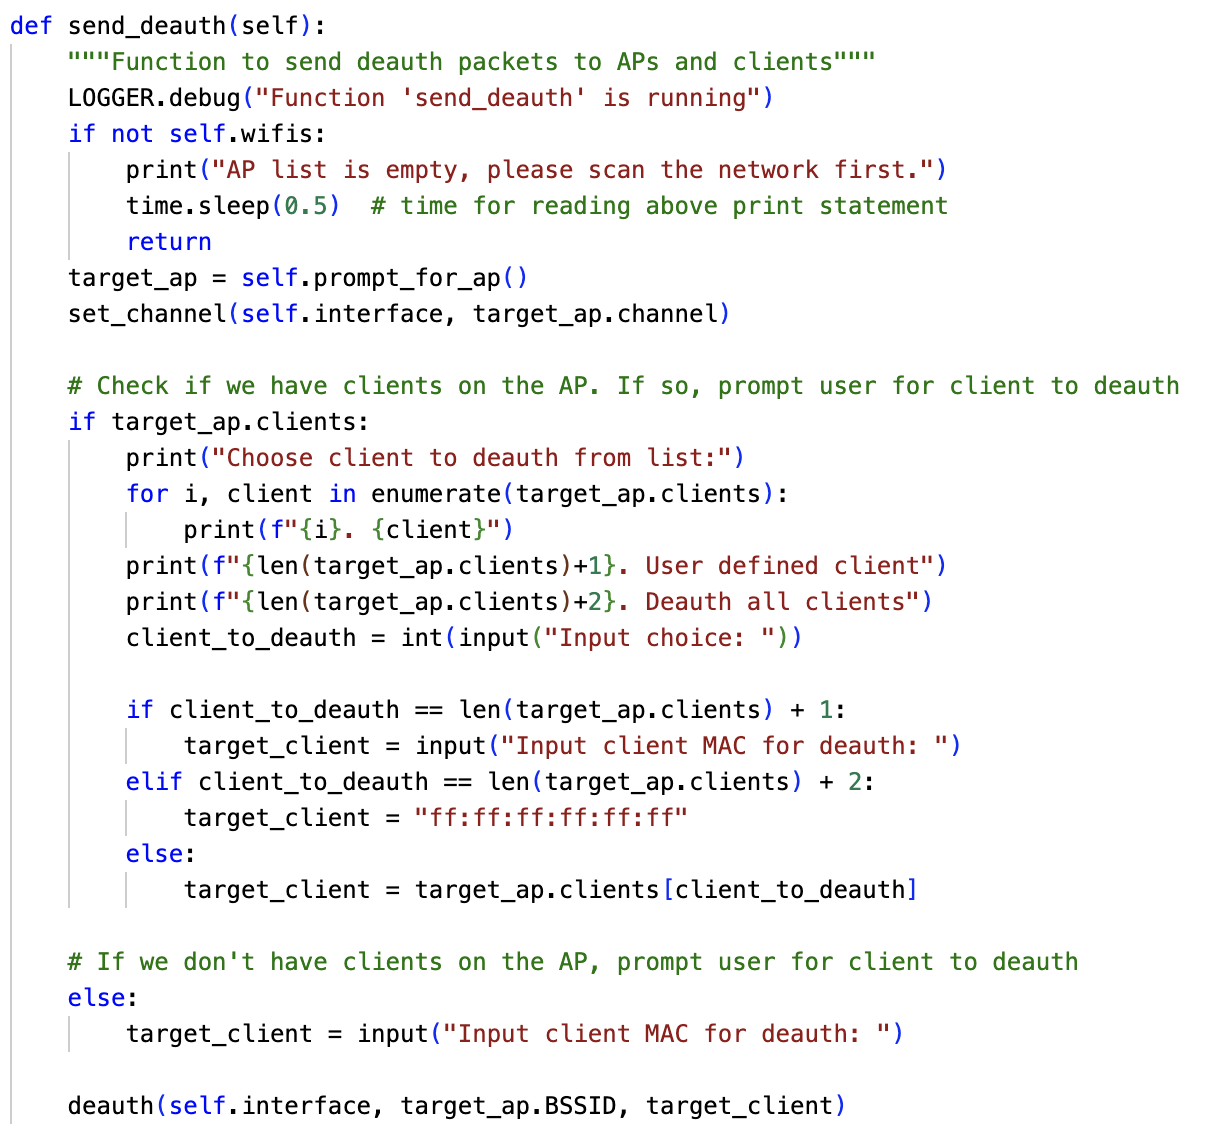
\includegraphics[width=\textwidth]{Latex-Files/Billeder/Implementation/deauth_prompt.png}
         \caption{Code for prompt and call of attack}
         \label{deauth_prompt_code}
     \end{subfigure}
     \hfill
     \begin{subfigure}{0.49\textwidth}
         \centering
         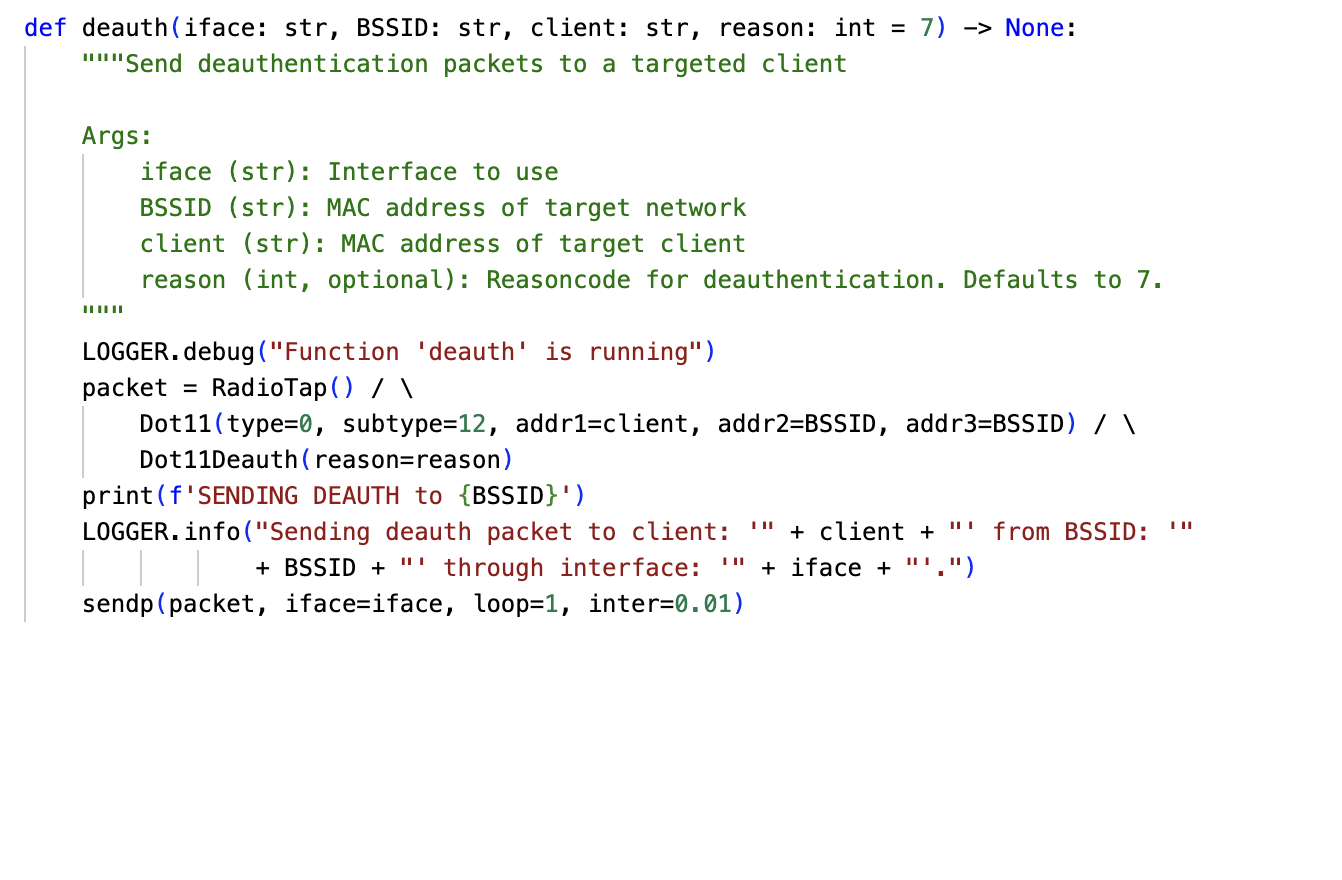
\includegraphics[width=\textwidth]{Latex-Files/Billeder/Implementation/deauth_packets.png}
         \caption{Code for deauthentication attack function}
         \label{deauth_func_code}
     \end{subfigure}
     \hfill
     \caption{}
\end{figure}

After a target AP and a target client has been defined, the "deauth" function, seen in figure \ref{deauth_func_code}, is then called. This function is what creates the appropriate deauthentication packets. The instantiation of the packet works by stacking layers on top of each other. In this case the packet is created by first making a RadioTap layer, which is responsible for sending the packet we create.

Then a Scapy "Dot11" layer is made, which represents a basic 802.11 frame. Here the type i set to 0, indicating a management frame, and the subtype to 12 indicating a deauthentication frame. From here the addresses are defined for the target of the frame. 

Finally the last layer is added, this being the "Dot11Deauth" layer which here defines a reason code for the deauthentication. This reason code is set to be 7 by default, which corresponds to the reason "Class 3 frame received from non-associated STA" \cite{Cisco_Deathentication_reasoncodes}. In a communications relation, the reason code provides important information about the cause of the deauthentication. However it is not an integral part of the deauthentication action itself, therefore the reason code is just given as a random number we have chosen.
Although it does not have a functional use, the reason code could in practice improve a deauthentication attack, by using appropriate reason codes, thus further concealing the fact that it is of malicious nature.

Subsequently a line is printed to the console notifying the user that a deauthentication attack will commence, combined with the target for the attack.
Ultimately the "sendp" function sends the beforehand created deauthentication frame on the second layer of the OSI model. Since this is where the deauthentication frames are transmitted\cite{data-link-layer}.


Figure \ref{deauth_attack} shows the output presented to the user, when performing the deauthentication attack. The user can here choose to selectively deauthenticate a single client. Alternately the user possesses the option to deauthenticate all clients from the targeted AP. Upon the user inputting a choice, the program begins transmitting the packet constructed. The deauthentication attack is continuous and will only stop when interrupted by the user. Using the keyboardinterrupt, as seen done in figure \ref{deauth_attack}. 

\begin{figure}[H]
    \centering
    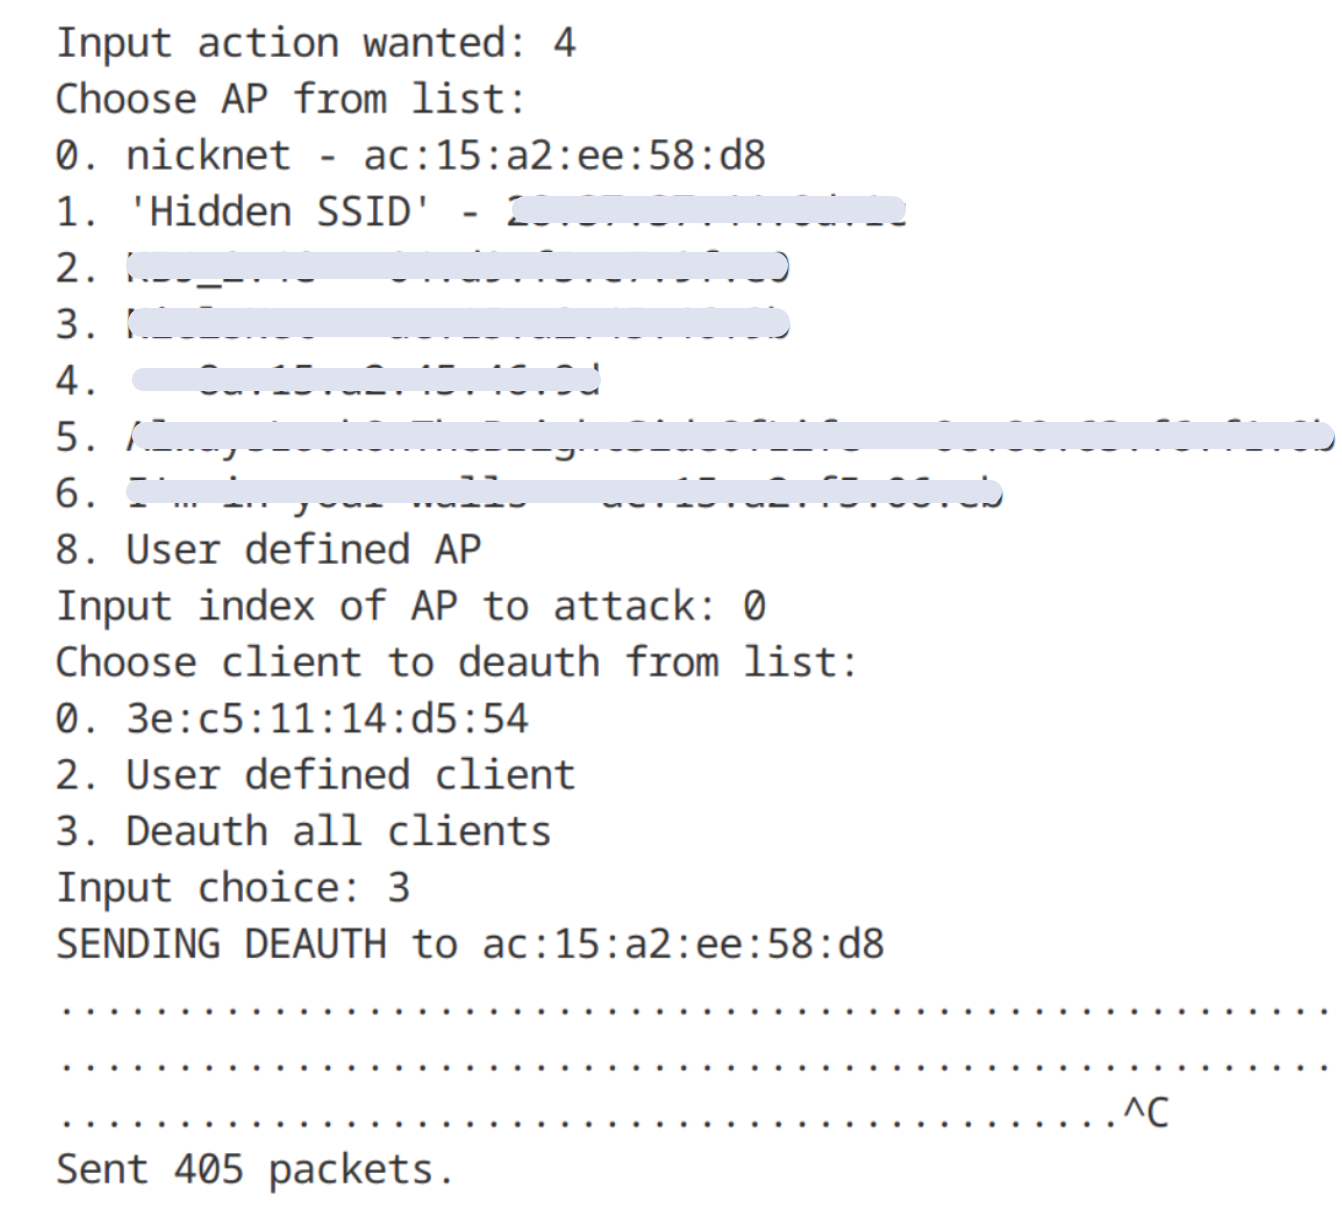
\includegraphics[width=0.5\textwidth]{Latex-Files/Billeder/Implementation/deauth_attack_censored.png}
    \caption{Output when performing deauthentication (blurred for privacy reasons)}
    \label{deauth_attack}
\end{figure}

Notice the SSID of AP nr. 1 in figure \ref{deauth_attack}, this is a hidden SSID, which is caught by the program, and set to "'Hidden SSID'".

\subsection{Password cracking}
The implementation of password cracking uses Scapy to read and save packets being sent on specific channels. It uses the implementation of the WiFi-scanner to get the APs that have the potential to be cracked. The function is as follows:

First a menu is shown where the user can chose between scanning for packets and cracking with the packets. If scanning is chosen, then the user is, like with deauthentication, shown a table of known APs as seen on figure \ref{WEP_code1}. The user then chooses which AP to crack. If an AP without WEP is chosen an error occurs as seen on figure \ref{WEP_code2}. If not, it begins to sniff packets on that AP's channel and saves every packet that contains a WEP part. This is done for a specific amount of time as chosen by the user. 

\begin{figure}[!htbp]
     \centering
     \begin{subfigure}{0.49\textwidth}
         \centering
         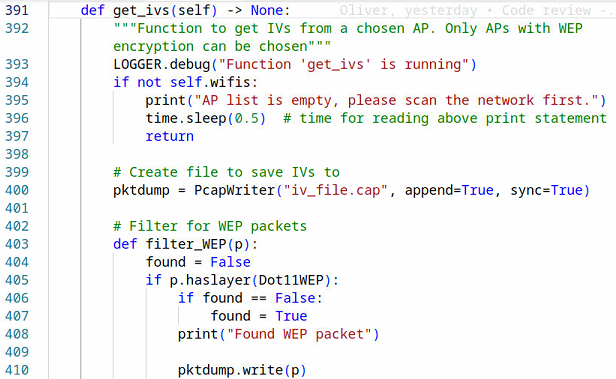
\includegraphics[width=\textwidth]{Latex-Files/Billeder/Implementation/Code1.png}
         \caption{Code for WEP filter}
         \label{WEP_code1}
     \end{subfigure}
     \hfill
     \begin{subfigure}{0.49\textwidth}
         \centering
         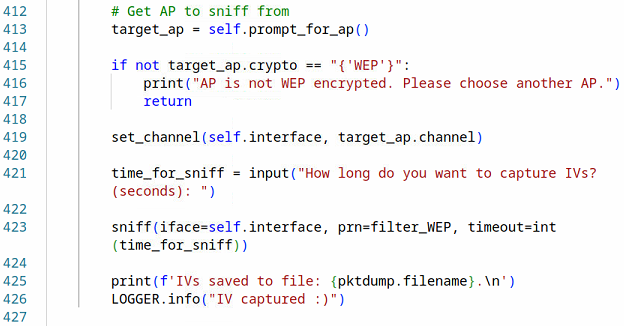
\includegraphics[width=\textwidth]{Latex-Files/Billeder/Implementation/Code2.png}
         \caption{Code for sniffing of packets}
         \label{WEP_code2}
     \end{subfigure}
     \hfill
     \caption{}
\end{figure}


Afterwards the packets are saved in a file that can then be read by Aircrack-ng. Aircrack-ng is run in a terminal on the file "IV\_file.cap.

Aircrack-ng is made up of commands that is used to manipulate data, it is not code written directly. This has the consequence that most of the implementation will be in the mapping of networks part. 

The way Scapy saves the packets has the consequences that Aircrack-ng cannot use the PTW method of cracking for passwords and subsequently it uses the lesser method, FMS, which requires a minimum of 250.000 packets, about 15 times more packets \cite{Weakness}. Therefore it needs a lot more time to crack the network. 


A successful test has also been completed with the use of Airodump-ng which is a part of Aircrack-ng.

\section{Tests}
In the testing of the product, multiple tests have been performed, these include both quantitative and qualitative tests. 
\subsection{Mapping of networks}
We have done a good amount of testing of our program. First we tested the mapping of networks as that is a requirement for the deauthentication. 

We tested on DTU campus, which should give us APs that are connected to DTUsecure, eduroam, DTUdevice and DTUguest. It should also give us all clients nearby as their MAC address. The result is shown on figure \ref{test1}.

\begin{figure}[!htbp]
    \centering
    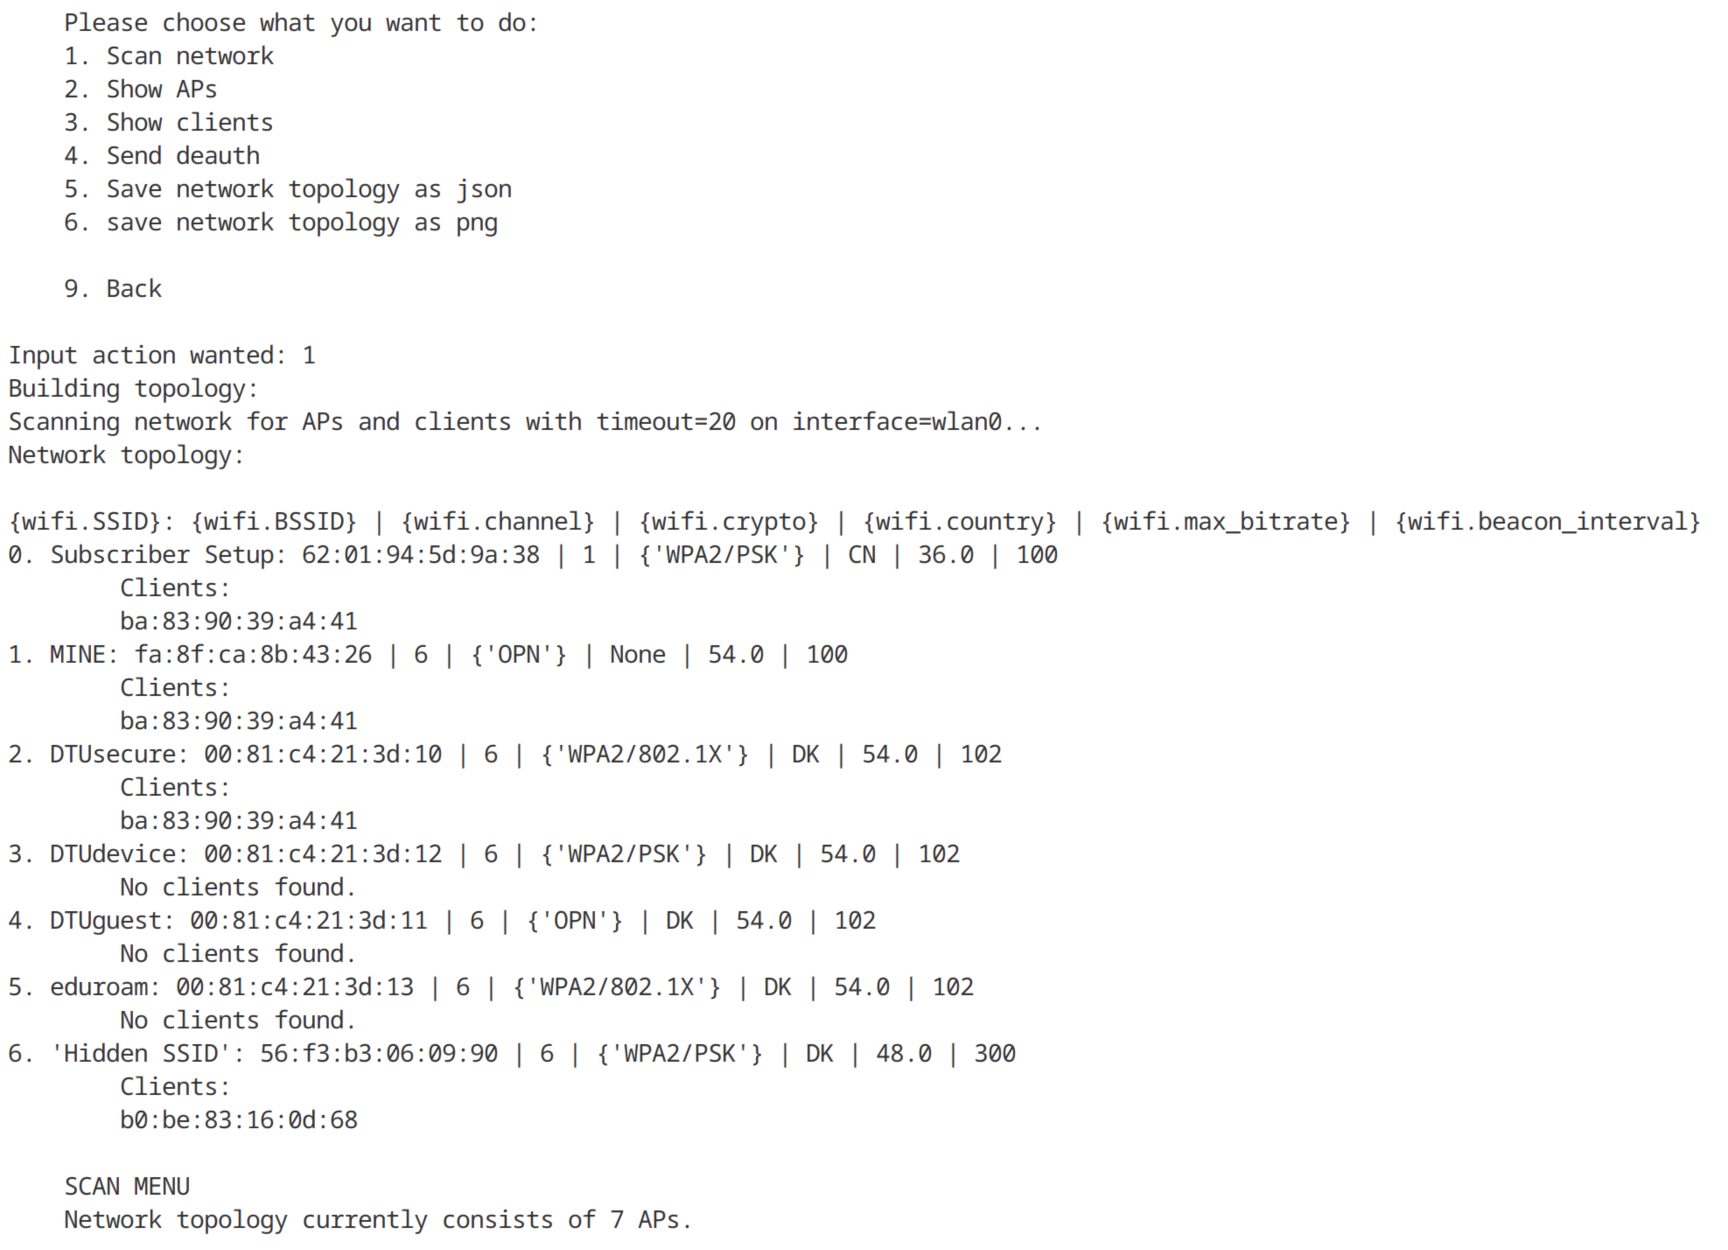
\includegraphics[width=\textwidth]{Latex-Files/Billeder/Tests/scan_network.png}
    \caption{Testing the network mapper}
    \label{test1}
\end{figure}

As we can see the test was successfully completed and DTUsecure, eduroam, DTUdevice and DTUguest showed up, together with some other APs unconnected to DTU. We have also found clients nearby. This shows that the mapping of networks has been successfully implemented.


\subsection{Deauthentication}

The deauthentication of a Macbook was tested. It was connected to a smartphone set up as an AP (using WPA2) and both the Macbook and the AP showed up. We started a constant ping on the Macbook and afterwards started the deauth attack. The pinging i shown on figure \ref{Test2}.

\begin{figure}[!htbp]
     \centering
     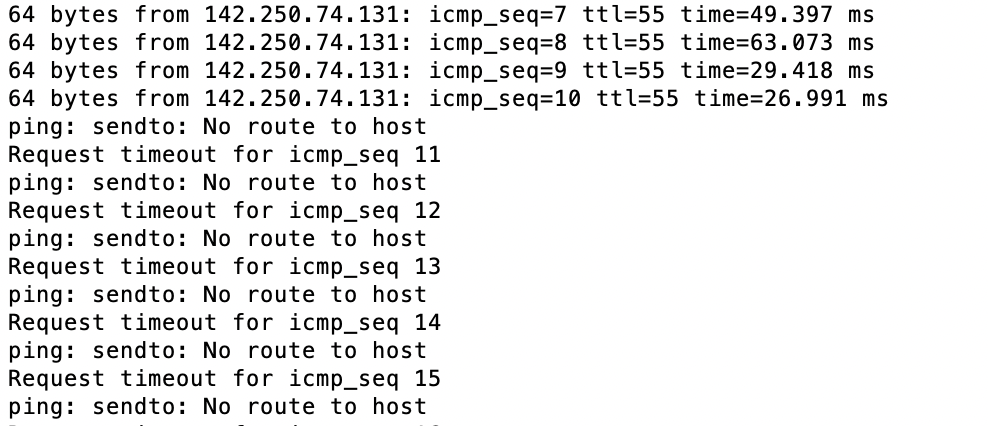
\includegraphics[width=0.5\textwidth]{Latex-Files/Billeder/Tests/deauth_ping.png}
     \caption{Result from being attacked (Mac)}
     \label{Test2}
\end{figure}

Figure \ref{Test2} shows the result of the attack. This attack was run by deauthenticating a single client. it is evident that the pinging to google works in absence of complications, however when the deauthentication attack is deployed, the pinging encounters issues and outputs "No route to host". Thereby denying the client service, and disconnecting the client from the internet. We then tested on a Windows PC as seen on figure \ref{Test3}.

\begin{figure}[!htbp]
    \centering
    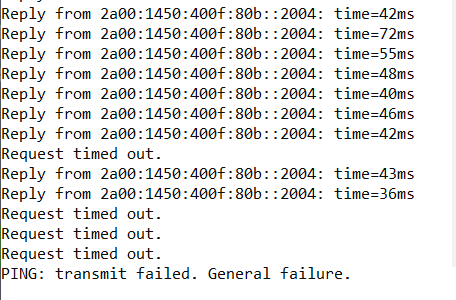
\includegraphics[width=0.5\textwidth]{Latex-Files/Billeder/Tests/Deauth virker.png}
    \caption{Result from being attacked (Windows)}
    \label{Test3}
\end{figure}

As with the test on the macbook, it is here evident that a stable connection is in place in the beginning. Whereas once the deauthentication attack is deployed, the connection is interrupted. Thereby showing that the deauthentication attaack works on both the Windows and Mac operating system.

\begin{figure}[H]
    \centering
    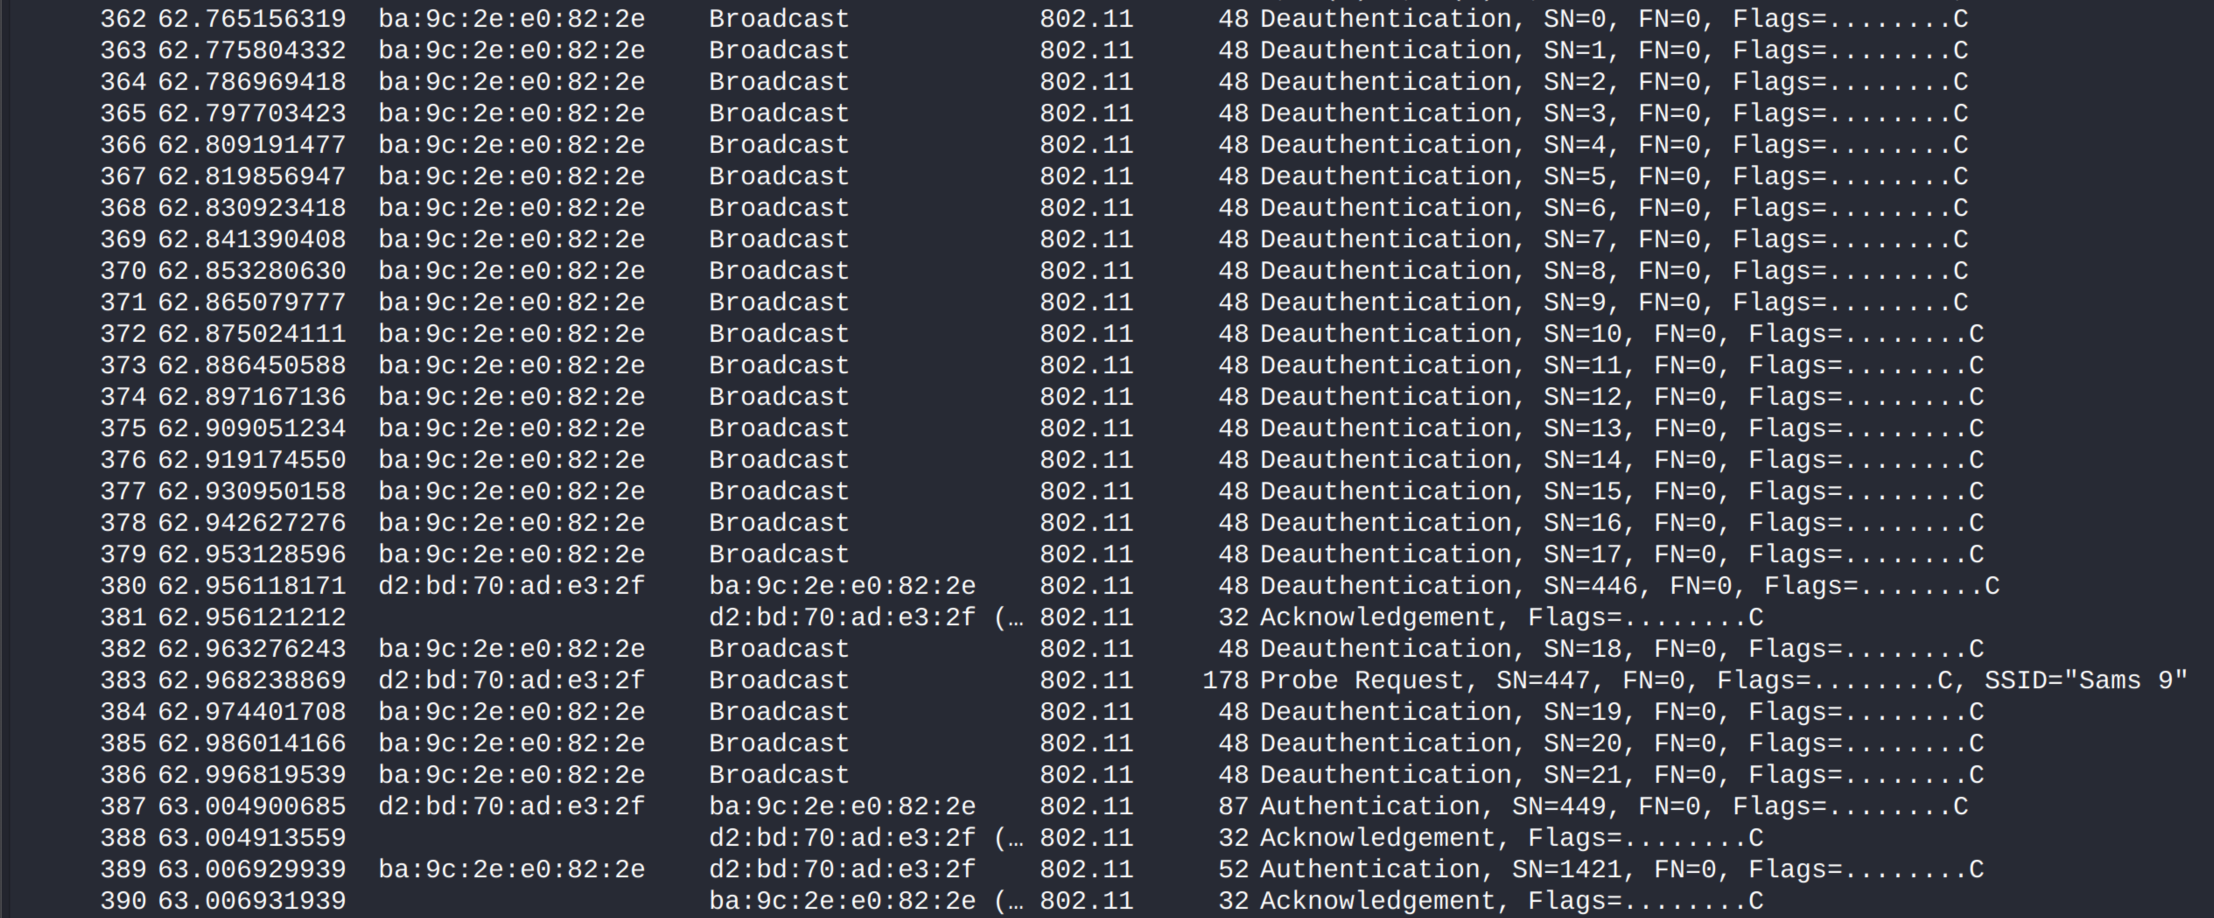
\includegraphics[width=0.7\textwidth]{Latex-Files/Billeder/Tests/deauth_pcap.png}
    \caption{pcap of deauthentication}
    \label{deauth_pcap}
\end{figure}

As well as testing the deauthentication by pinging, we have examined the packets themselves using Wireshark. In figure \ref{deauth_pcap} the deauthentication packets sent out can be observed. It is evident that as expected, our program transmits deauthentication packets for the designated target. The deauthentication packets were, in this test, broadcasted in order to deauthenticate all clients connected to the AP. 
Notice packet number 381, which is an acknowledgement, thus confirming the deauthentication of the client.


\begin{figure}[H]
    \centering
    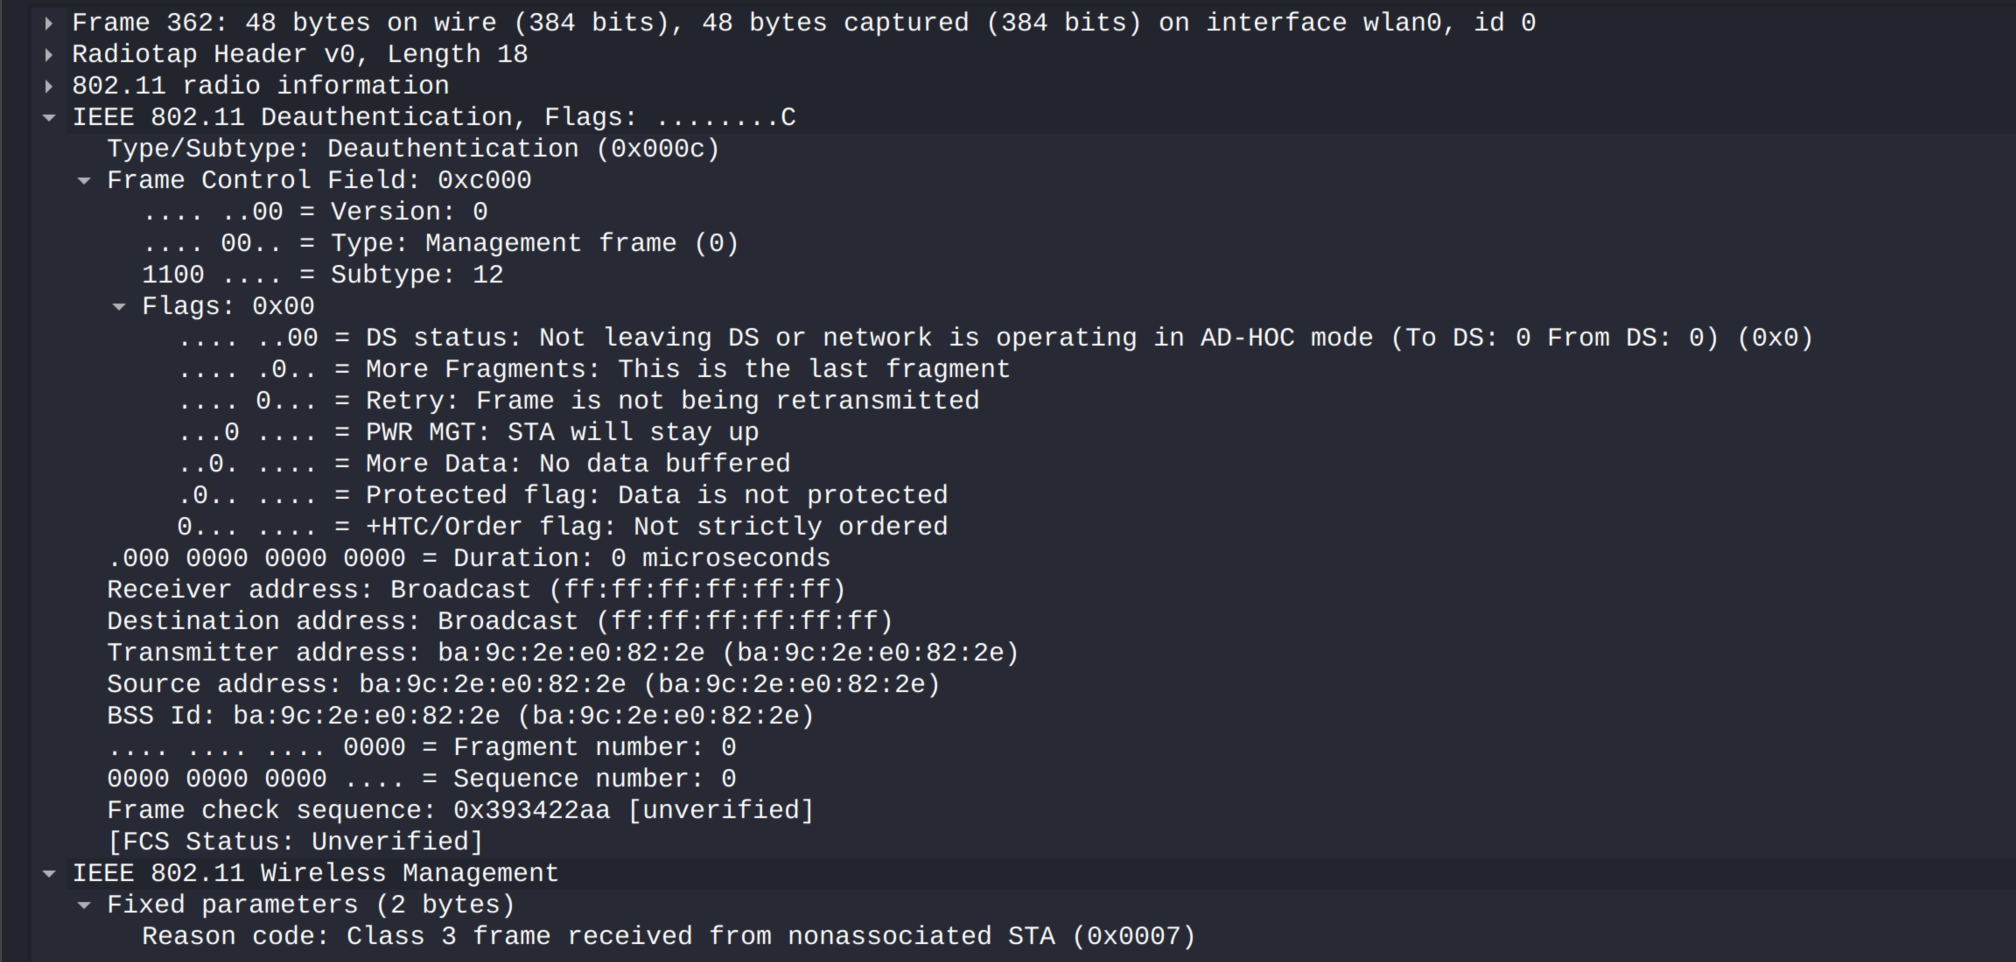
\includegraphics[width=0.7\textwidth]{Latex-Files/Billeder/Tests/deauth_pcap_packet.png}
    \caption{Deauthentication packet further inspection}
    \label{deauth_pcap_packet}
\end{figure}

Delving deeper into a particular deauthentication packet transmitted, as shown in figure \ref{deauth_pcap_packet}, we can observe the specific parameters set during the deauthentication. The receiver, and destination addresses are both set to the broadcast address, and the source address is set to the AP the clients will be disconnected from. Additionally the aforementioned reason code for the deauthentication is shown as reason 7.


\subsubsection{Examination of deauthentication frame interval}
Examining the test on frame interval, with results seen in table \ref{Examination of deauthentication frame interval}, as standpoint, the interval in which each deauthenticaion frame is sent from the attacker is examined in order to propose an ideal interval. The setup has been tested outside for the minimal amount of interference and reflection from surface areas and has been done with the wireless dongles Qualcomm Atheros UB93 and the Realtek DWA 131-E1 for the attacker and defender respectively in order to simulate a likely setup. For the first test, the distance was 1 meter between the users, such that distance would not affect the result. The test parameters was a qualitative answer to if the user was successfully deauthenticated and how many packets was sent and how many where received and the loss. The resulting data can be seen in table \ref{Examination of deauthentication frame interval}.

\begin{table}[!htbp]
\centering
\begin{tabular}{lllll}
\hline
Interval & Deauthenticated? & Packets send & Packets recieved & Loss     \\ \hline
0,001    & y                & 714          & 133              & 0,813725 \\
0,005    & y                & 1952         & 413              & 0,788422 \\
0,01     & y                & 1325         & 343              & 0,741132 \\
0,05     & y                & 822          & 191              & 0,76764  \\
0,5      & y                & 45           & 12               & 0,733333 \\
0,8      & n                & 52           & 7                & 0,865385 \\ \hline
\end{tabular}
\caption{Test of deauthentication packet transmission interval}
\label{Examination of deauthentication frame interval}
\end{table}

From the data it can be extrapolated that the packet loss is generally the same for all intervals, which makes sense as it should mostly depend on distance. Likewise it is seen how the client was deauthenticated until the 0.8 second interval. It should also be noted that, while running the test, it was clearly seen that more packets where sent during the 0.005 second interval than during the 0.001 second interval. This might have been caused by the hardware not being able to send packets this fast and should be further tested with more types of hardware. The attack had, from a qualitative point of view, much more success when using a lower interval. Yet this is problematic as the attack is now much more visible to WIDS (wireless-intrusion-detection-systems). Thus it would be better for an attacker attempting to hide in plain sight to use an interval of 0.5 as this is still successful at deauthenticating clients.

\subsubsection{Examination of deauthentication with variable distance}
Afterwards the attack was repeated with a constant interval of 0.005 seconds as that was shown to be the most optimal choice in a cost vs. risk assessment. Now the variable was distance, starting at 1 meter up to 15 meters. The resulting data is shown on table \ref{Examination of deauthentication with variable distance}.

\begin{table}[!htbp]
\centering
\begin{tabular}{lllll}
\hline
Distance {[}m{]} & Deauthenticated? & Packets send & Packets recieved & Loss     \\ \hline
1                & y                & 1096         & 224              & 0,79562  \\
5                & y                & 1884         & 177              & 0,906051 \\
7,5              & y                & 1499         & 200              & 0,866578 \\
10               & y                & 1504         & 141              & 0,90625  \\
15               & n                & 1248         & 72               & 0,942308
\end{tabular}
\caption{Test of deauthentication performance by distance}
\label{Examination of deauthentication with variable distance}
\end{table}

\begin{figure}[!htbp]
    \centering
    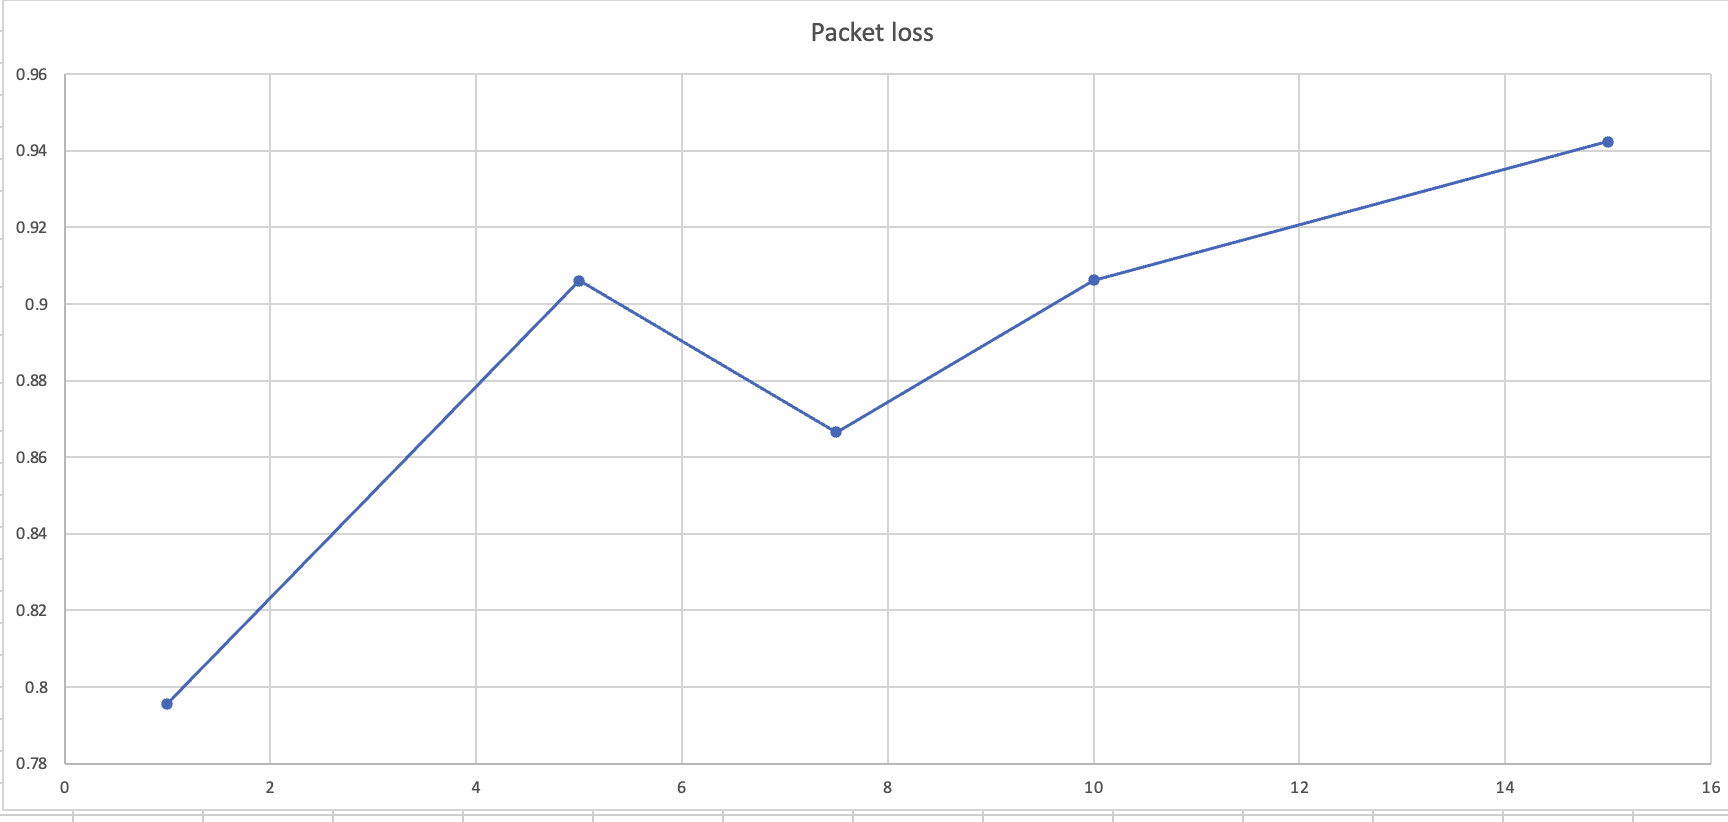
\includegraphics[width=0.7\textwidth]{Latex-Files/Billeder/Tests/deauth_afstand.png}
    \caption{Deauthentication packet loss(y) by distance(x)}
    \label{Packet loss graph}
\end{figure}


It is evident that the distance is clearly affecting the loss ratio: The further away the attacker is from the target, the worse the attack performs, and at 15 meters and above, the attack completely fails at deauthenticating the client. This further validates the vulnerability of the attack type in that the main requirement is that the attacker is very close to the client and that this places limitations on the attack thus further segmenting it as an on-premise attack.

The very high packet loss, at minimum 75\%, for both tests, regardless of distance or interval is caused by the environment affecting the setup (reflections, temperature, humidity etc.), but the most significant factor is the channel changing implementation. The program is set up to switch channels every 0.205 seconds as explained in the implementation and as a consequence, the client only receives deauthentication packets when the attacker is on the same, or surrounding, channels as the client, which accounts for approximately 4 to 5 channels. Backhanded math shows that this equals about $\frac{5}{14} = 35\%$ of the channels and thereby about 35\% of the time and so a minimum of 75\% of the packets are lost, which is clearly shown in test and the rest is accounted for by the environmental impact.

\subsection{Password Cracking}
Two tests where done for password cracking, one only using Aircrack-ng to test if our AP was compatible and if Aircrack-ng works. The second test was about if our program could get the required IVs to make Aircrack-ng crack the WEP protected AP.

\subsubsection{Test 1: Aircrack-ng only}

This test was only using Aircrack-ng and Airodump-ng, a subfunction of Aircrack-ng, to collect packets and crack the AP.

\begin{figure}[!htbp]
    \centering
    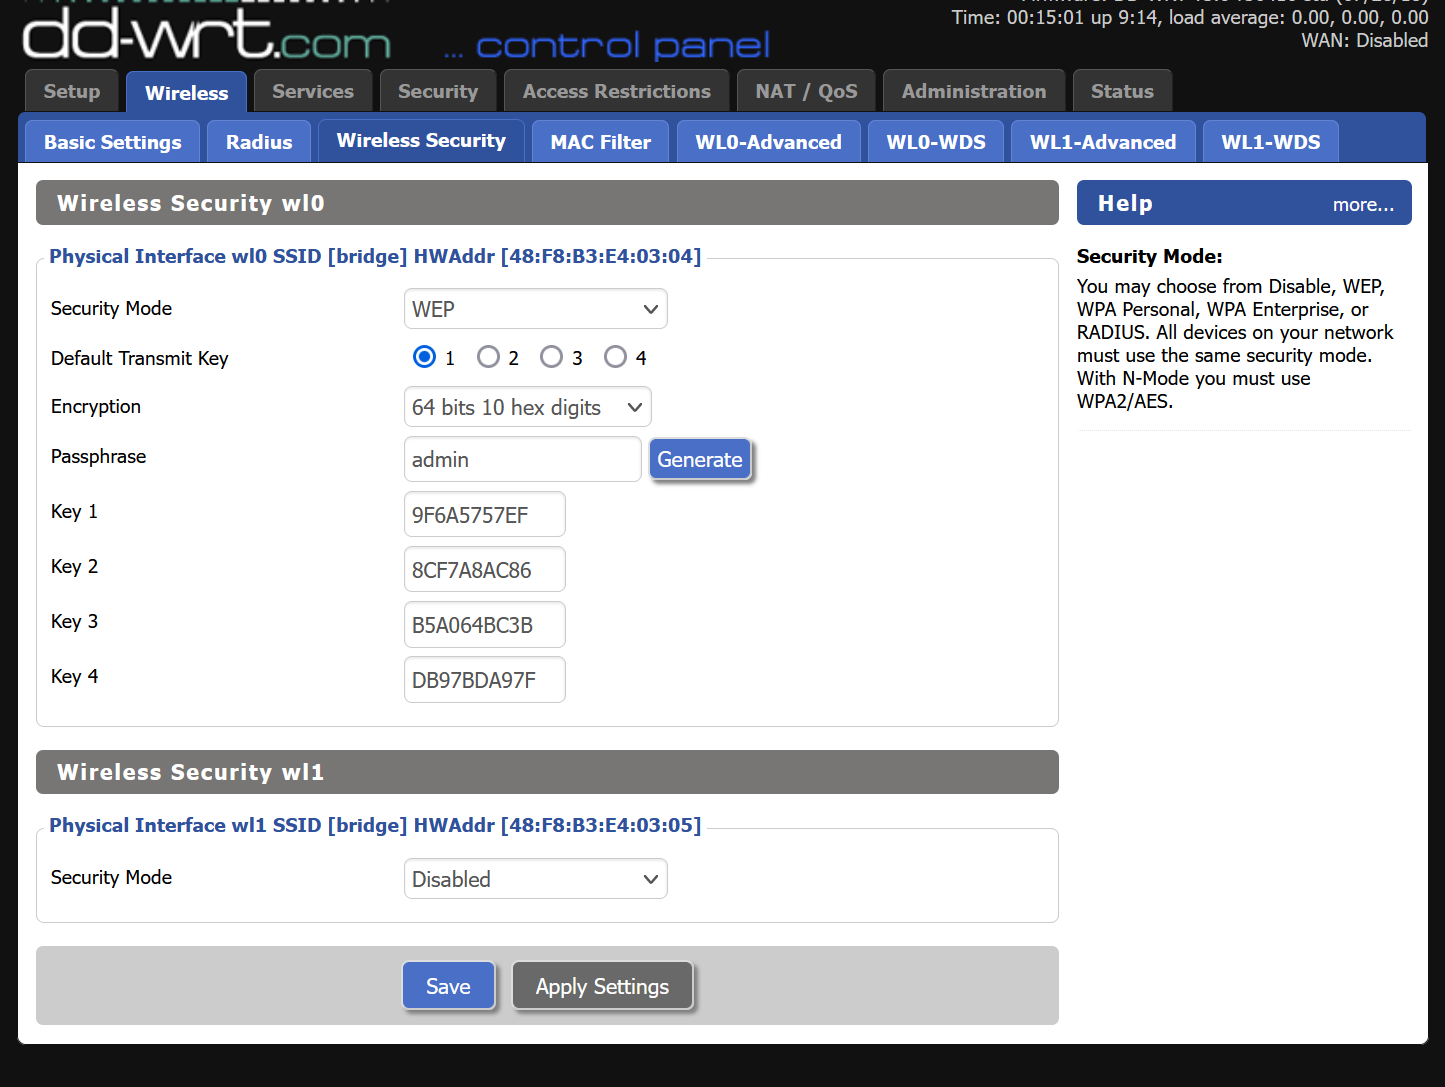
\includegraphics[width=0.5\textwidth]{Latex-Files/Billeder/Kode2.png}
    \caption{The passwords on the AP}
    \label{Crack2}
\end{figure}

The test was that an AP, with the capability to use WEP, was set up and connected to a wider network on the internet and then made to use WEP with passkeys, as seen on figure \ref{Crack2}. Then a computer using Linux was connected to that AP and a constant stream of data was created by watching YouTube. Then another computer was setup to monitor these data-packets and capture those that contain an initialization vector (IV). 

There was a small problem with the connection between the AP and the wider internet, so we had to constantly pull the Ethernet plug and replug. This was probably because the wider network didn't like using WEP, and that was also why YouTube did not actually work. So the computer sent and received data-packets from the AP only. Enough data-packets where still created and so a large .pcap file was made with about 10.000 IV packets. 

\begin{figure}[!htbp]
    \centering
    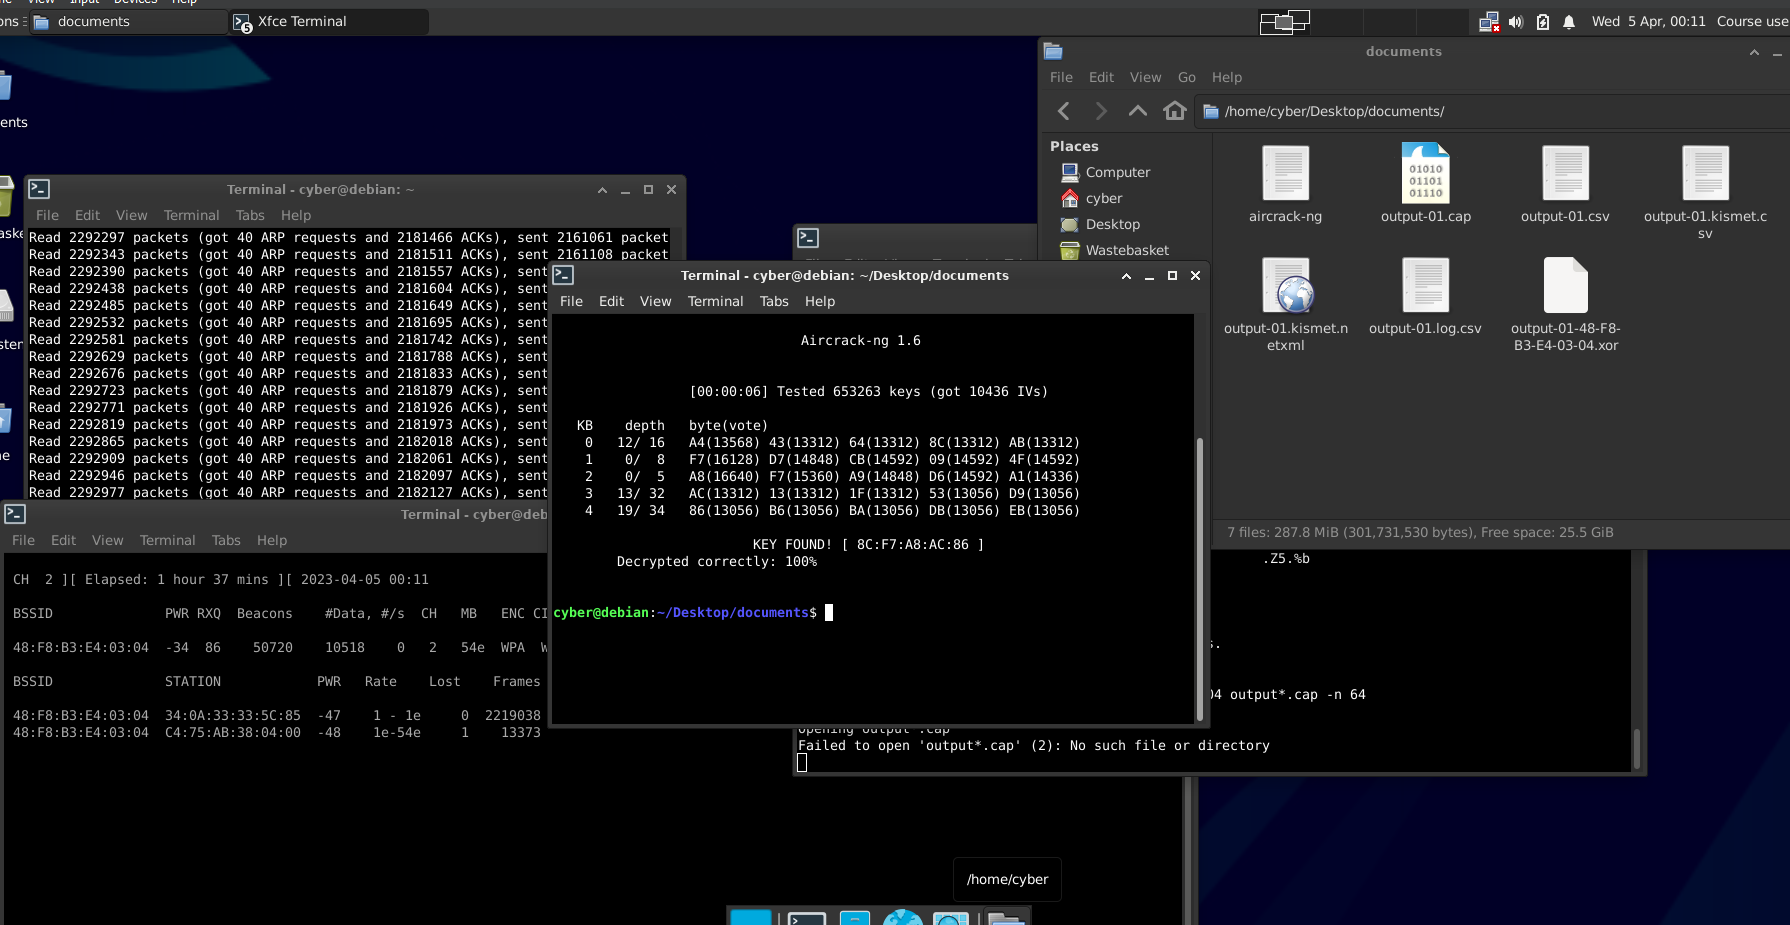
\includegraphics[width=0.5\textwidth]{Latex-Files/Billeder/Kode1.png}
    \caption{Aircrack-ng finding the password}
    \label{Crack1}
\end{figure}


Then Aircrack-ng was used on this .pcap file to find the passkey, which it did after 40 seconds. The passkey corresponds with one of the chosen passkeys on the AP. We can see the result on figure \ref{Crack1}.

Next a test was done using the programs \lstinline{get_ivs} function on the same AP with a different password. The options of the AP is shown on figure \ref{Crack3} 
\begin{figure}[!htbp]
    \centering
    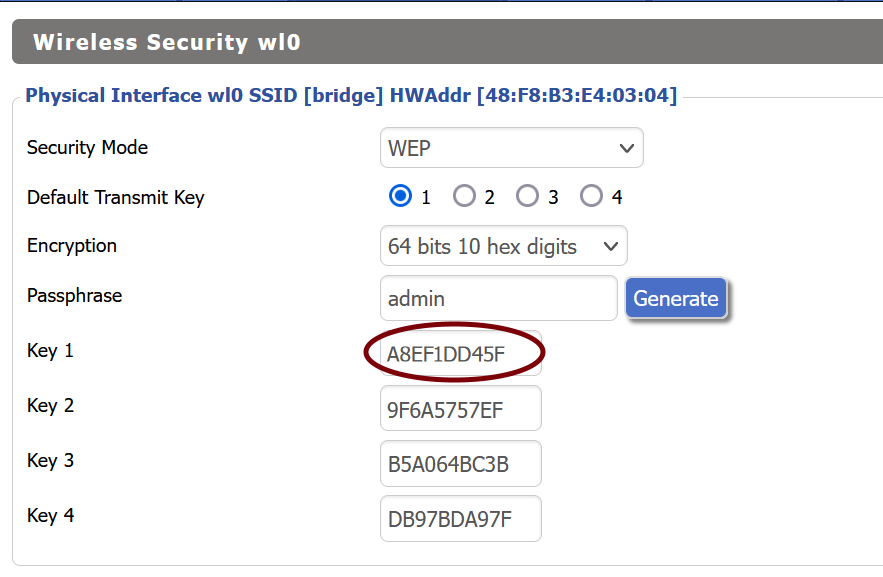
\includegraphics[width=0.8\textwidth]{Latex-Files/Billeder/Tests/WEP1.png}
    \caption{Aircrack-ng cracking the password in test 2}
    \label{Crack3}
\end{figure}

A computer was connected to this AP that was connected to the internet and a Youtube video was initiated and the function was ran on another computer with the dongle inserted for about 10 minutes. This gave it about 150.000 IVs.

\begin{figure}[!htbp]
    \centering
    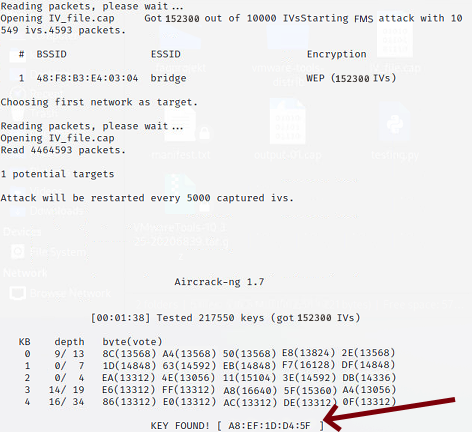
\includegraphics[width=0.5\textwidth]{Latex-Files/Billeder/Tests/WEP2.png}
    \caption{The password on the AP in test 2}
    \label{Crack4}
\end{figure}

Now the crack could be started on Aircrack with the FMS attack and it took a minute longer to complete and gave the correct code out. This shows that our program can be used to get the IVs required to crack a WEP protected AP.

\section{How to Run}
This section highlights requirements to run the program, as well as outlining how to run the program. 

An example run of the system has been recorded and uploaded to YouTube as a guide for the user, watch it here:
\url{http://youtu.be/MvI8mlnKXYc}

The program has a repository on GitHub, which can be accessed through the link underneath.
\url{https://github.com/s214684/fagprojekt}
\subsection{General Requirements}
The program must be run on a Linux system. If run on a windows or mac, the program will raise an exception, and terminate the program. Furthermore the user must run the program as root ("sudo"), if not the program will terminate.
Lastly the user must have a network card capable of monitor mode, if not the program will terminate.
\subsection{Network Scan}
Most functionalities of the program require a populated map of the network, this is achieved by scanning the network. 
Start the program by running the "\_\_main\_\_" file as root. Then the user is prompted with 4 options.
To scan the network, input "1" and press enter.
The program will now scan the network, and populate the topology.
Upon finished scanning, the user is shown the discovered topology of the network, as well as more actions. This is seen of figure \ref{test1}.
When the network has been scanned, the user can at any time scan the network again, thus further populating the already known topology.
\subsection{Deauthentication}
When the network has been scanned, the user has the possibility of launching a deauthentication attack on a known AP. To do this navigate to the "send deauth" option in the menu after scanning the network.
Press "4" and choose which AP to deauthenticate.
When an AP has been chosen, the user has the option to deauthenticate a known client, input a user defined client, or send to all clients.
When a client is selected, the deauthentication packets will be sent indefinitely, the user can now interrupt the deauthentication by pressing "CTRL+C", this ends the transmission and sends the user back to the program.
\subsection{WEP Password Crack}
Back at the main menu the user can now choose the Crack WEP option. In this menu the user can choose between choosing an AP to scan or cracking their WEP. Choosing an AP to scan shows all local APs and allows the user to choose which AP to scan, only WEP encrypted networks are eligible for the attack, as that is what our program works with. Then the user can choose how long he/she wants to scan, the program will warn the user once the first WEP packet has been detected, thus ensuring the user knows whether the crack is running as intended.

The user can subsequently choose to crack that AP, however, since the program is purely integrated to work with Aircrack-ng, the user will be suggested to open Aircrack-ng themselves. This is done by installing Aircrack-ng on Linux and then running a terminal where the file iv\_file.cap is located and running the command: "sudo aircrack-ng iv\_file.cap" thereby attempting a crack on the WiFi.
\subsection{Options}
From the main menu, the user can go to the options menu. Wherein he/she can choose between the timeout, which defines the time for scanning for packets to populate the network topology. The default is 7 seconds, which should be enough to get all APs and some clients if they are active on the network. If not, the user can set a longer timeout. The user can also choose another interface in case he/she has multiple interfaces set up. This is only recommended for advanced users as the default should work.

\section{Discussion}


\subsection{Main Challenges}

During this project the main challenge was that internet traffic is complicated and made up of many interlocking parts. There is a lot of data being sent and much of it is not relevant to what we are doing. As we worked with a shared medium, it was hard to differentiate between what data we create with our program and what is part of standard internet traffic. This made it difficult to figure out what was going on 'under the hood' when we where testing our implementations. Consequently it took far longer than needed to do some of the basic mapping of the network and simple deauthentication. Still, this was very much a learn-by-doing project in that we obtained solutions to tackle or overcome the problems and implementing our WiFi-scanner we have gained valuable knowledge about how data-packets are built. 

Likewise the theory behind most of the 802.11 management frames and such used in this project was very new to us, since only a short overview of 802.11 has been provided in our courses where the focus mainly has been on the EAPOL 4-way-handshake within WPA. Thus, at the start, there was a great gap in knowledge that we had and what we needed as some of the implementation required deep understanding of how e.g. the procedure for deauthentication works.

When cracking WEP, the main challenge was figuring out how to get the right packets from the right source consistently and enough of them so that enough IVs could be found for Aircrack. The challenge of actually cracking the WEP algorithm was to big to solve within the scope of this project (as the main goal has been deauthentication and mapping of the network), this was the reason for the usage of Aircrack.

We also had to work hard to make the code understandable for outsiders and so we focused a lot on that at the end, by rewriting and removing parts we did not use. 


\subsection{Future Work}
For continuing our work we could possibly implement our own WEP cracking algorithm, so that we would not be dependant on Aircrack. This would mean that we would have to understand and be able to implement the FMS attack completely which would be a project in and of itself, but possible. We could use one of the two types of attacks cited in the paper Fluhrer, Mantin \& Shamir \cite{Weakness}.

As mentioned under the test section it can make sense to create a mobile system capable of using the developed tool in order to easier exploit victims. This is due to the fact that the attacker thus can remove herself from proximity of the victim making disclosure of the attacker harder. Therefore it would make sense to build a mobile system, capable of running for extended periods of time. It can here also be examined whether a direct connection to the attacker is required to send information about the reconnaissance and attack instantaneously - which would further expose the attacker as these signals could be obtained/exploited by a defender. Yet if no direct communication is possible, the attacker would need to return to the device in order to obtain the information. We propose a solution in which telecommunication is exploited as this in general is harder to track for a common defender especially if the area in question is somewhat populated. Likewise a Raspberry Pie could be an ideal device with plenty of computational power to further elaborate on the toolset in the future.

Further improvement to the wifitool could be made in the channel changer. As mentioned in the test of the deauthentication attack. The channel changer runs while transmitting deauthentication packets, thus creating a scenario where about 35\% of the transmitted packets are actually sent on the correct channel. This could be improved by only running the channel changer during the scanning of the network, thereby ensuring the deauthentication is only on the correct channel. 

The mitigation and discovery of the implemented attacks could also be researched further. Possibly implementing a way of discovering a deauthentication attack, this could be done using Scapy, and checking for irregularity in the network. Furthermore machine learning could be used for further exploration in the topic of mitigation. 


\section{Conclusion}
In this project we have investigated network traffic by mapping local WiFi networks using python and the tool Scapy to show all APs connected and the clients connected to these networks. By obtaining knowledge of the WLAN it was managed to send deauthentication frames from a spoofed source address, hence doing a deauthentication attacks to disconnect one or more clients from using wireless networking. By doing this we gained advanced knowledge about different types of frames and subframes in the 802.11 standard as well as a thorough understanding of the attacks. The security algorithm in the 802.11, namely WEP has been examined and exploited to understand fundamental methods as statistical analysis to exploit flaws in the algorithm. Yet there is still work left in order to explore mitigations for the different attacks. Likewise there is work left in order to ensure stability and integrity of the attacks, and anonymity when performing the attacks.  
During this project we also increased our knowledge of python programming and networking toolboxes that use python, which gives a broad understanding of how packets are structured. 


\section{Appendix}

\section{Peer Feedback}
We received feedback about some theory that should be added about Scapy. We fixed this by giving more information about Scapy.
We also changed how we inserted our code snippets as a screenshot of dark code makes it hard to read, so we fixed it by adding the code inside the report as text. 
We added a small section after the introduction showing who wrote what as it was proposed in the peer-review in order to obtain a quick overview.

\section{Collaborative Experience}
Our collaboration revolved around an approach, in which we collectively tackled project tasks and thought about the most effective strategies for their execution. We then divided the workload among the three group members, allowing each individual to focus on specific components.
Afterwhich we merged our contributions into a coherent program. During this phase, we engaged in discussions, exchanging expertise and gaining a deep understanding of our respective work. These interactions secured a full understanding of the project as an entirety for the whole group.
Throughout the 13-week period, we generally stuck to our planned schedule, although we found ourselves working more than anticipated. As a result, during the subsequent 3-week period, our initial time estimates were somewhat conservative. Thereby giving us extra time for smaller features of the program, such as the logger.



\newpage

\listoffigures


%\newpage
%\section*{Functionel Description Report}
\tableofcontents
\newpage

\section{Abstract}
The projects fundamental goal is to explore and examine properties of 802.11. The focus will be on exploring how management frames can be exploited for malicious use and how this can be mitigated. The main focus is on how deauthentication attacks can lead to Evil Twin Attacks. Further a side focus will be on the different authentication protocols in regards to password cracking. Thus in this project it has been possible to scan and identify the local wireless networks in the area, by exploiting beacon and probe management frames. Hereby giving the ability to deauthenticate clients and emulating a rogue AP for the clients to connect to, hence achieving a man-in-the-middle like state. Lastly it has been possible to crack/obtain a WEP password by obtaining initialization vectors.


\section{Introduction}

Security in wireless networks has become increasingly important do to the rapidly expanding use and need for internet access. However, even with the many security measures in place for wireless networks, there are still vulnerabilities to attacks on said networks. One such attack is the deauthentication attack. Wherein a user will be rejected access to the network he/she is attempting to create a connection to.

This project will, explore the theory and practical applications of deauthentication attacks on networks. Furthermore we will investigate the cracking of passwords used in the encryption of wireless network traffic using the now outdated WEP protocol. To achieve this, we will need to gain knowledge of the wireless local area network (WLAN). Therefore another goal for the project is to create a table of available WiFi's, along with information on clients connected, signal strength etc.

Through this project, we aim to highlight the vulnerabilities of wireless networks and demonstrate the importance of securing them. It is important to note that this project is for educational purposes only and should not be used for malicious activities. Overall, this project will provide a comprehensive understanding of the above-mentioned vulnerabilities of wireless networks and how these might be mitigated/detected.

\iffalse
2 De tre søjler
2.1 Mapping af netværk
    Det skal være muligt at sige alt om sit WLAN:
    • hvor mange WiFi er der (herunder alle AP’s p ̊a hvert WiFi)
    • Hvor mangle klienter findes der (svært ved randomization af MAC (fint teori-afsnit))
    • Hvilken klienter er logget ind p ̊a hvilken netværk
    • Er MAC-adresse en klient eller AP (from-ds/to-ds)
    • Hvor langt/tæt p ̊a er de
    • Hvilke kanaler er meget i brug
    • Evt. s ̊arbarhedsscanning
2.2 Deauth (Evil Twin)
    Det skal være muligt at DoS:
    • Klient
    • AP
    • Kanal
    Ligeledes skal der udforskes, hvorvidt disse DoS kan mitigeres og/eller opdages. god
    at udfolde - henrik Hvis tiden er til det, vil det ogs ̊a være spændende at udnytte deauth til at
    tvinge klienter hen p ̊a et rogue AP (man-in-the-middle).
2.3 Password cracking og WEP/WPA2
    Her opsætter man at man kan bryde den lette password algoritme WEP og ogs ̊a at vise hvordan
    WPA2 forbedrer p ̊a sikkerhden i forhold til WEP. Den bliver meget teoretisk og der skal kommes
    ind p ̊a hvordan WEP og WPA fungerer. Man kan lave nogle matematiske udregninger der viser
    hvor langt tid det gennemsnitligt vil tage at bryde forskellige passwords i WEP og WPA2, som
    tydeligt viser at WPA2 er bedre. Der skal laves kode som bryder pakker med WEP sikkerhed,
    som vi nok selv har lavet, da WEP ikke længere bruges.
\fi

\section{Functionality}
Our project constists of the following functionalities:
\begin{enumerate}
    \item Scan the wireless local access  networks and identify clients/Access Points
    \item Deauthentication attacks
    \item Password cracking
\end{enumerate}

These functionalities aim to be the core of the product that will be created. The first functionality, scanning for local networks, is the most important one as that is the basis of all other functionalities.

A deauthentication attack is a type of denial-of-service attack that targets communication between a user and a WiFi wireless access point \cite{Deauth}. It exploits a feature of IEEE 802.11 wireless networks that allows devices to disconnect from a network by the deauthentication management frame \cite{Deauth_Wiki}.
A deauthentication frame tells a device to stop using the network. It can be sent by either the access point or the device itself. Normally, it is used for legitimate purposes, such as ending a connection or switching to another network.

However, an attacker can exploit this feature and send deauthentication frames to the access point with a spoofed client source address. This causes the spoofed device to lose its connection and try to reconnect. This exploitation has multiple use-cases. If done repeatedly or to multiple devices, this can disrupt or disable the network entirely, thus resulting in a Denial-of-Service (DoS) Attack. Meanwhile it can also be used to obtain a EAPOL 4-way-handshake for WPA or as a way to misguide a client to a rogue access point created by a malicious user to obtain a Man-In-The-Middle state. 

The last point is password cracking. The product should be able to crack basic passwords in the WEP algorithm as that is one of the most basic security algorithms. It is an outdated and non secure algorithm and the product can use some of the multitude of tools available to crack it, such as Aircrack-ng's PTW and FMS or WEPcrack \cite{aircrack-ng}. Alternatively we can create our own algorithm for cracking WEP if the time permit.

The implementations are mainly based on the python library Scapy to implement the functionalities \cite{scapy}. As our network interfaces has to be put in monitor mode a UNIX environment is used. The plan is to use a raspberry pi later in the project to obtain mobility and a uniform platform if time permits. 
The network interface is a Realtek DWA 131-E1 dongle as it is cheap and allows for monitor mode. The UNIX platform has the consequence of limiting the use of the implementation to a specific operating system. Though this should be able to be ported to Windows if need be. Here the Linux-sub-system on Windows might be exploited.
The positive side of using UNIX is that we can implement the program on many types of systems as we use a virtual machine to create the product. Thus making conversion to a raspberry pi easier. The negative side is that we have to use a virtual machine which can create problems with drivers and performance. 

\section{Blocks and sub-blocks}

This project will be built on 3 main blocks, "Mapping of networks", "Deauthentication" and "Password cracking". In in these blocks will be sub-blocks containing functionality for the specific block. 

\subsection{Mapping of networks}
This block takes the physical data being sent in the wireless space, and transforms it into information that the other blocks need and use. It contains a table that holds the information as sub-blocks, for instance access points (AP) in the WLAN, as well as the clients on said AP. Or the signal strength of the AP and which channels are used. This mapping can be done via beacon management frames used by APs to announce their respective presence. Likewise probe management frames can be used to understand what APs a client has been associated with in the past.

\subsection{Deauthentication}
This block handles deauthentication, wherein we deny clients access of certain AP's or all wireless internet usage. Thus making the sub-blocks: 
\begin{itemize}
    \item Client
    \item AP
    \item Channel
\end{itemize}


\subsection{Password cracking and WEP/WPA2}
This block is mainly about WEP and how to crack it, although this also tackles how generally secure passwords are for WEP vs WPA2. There is a high probability that this block also contains some way of creating packets with encryption, as packets with WEP are very uncommon since the widespread release of WPA and beyond.


\section{Theory}
The main theory behind this project is the 802.11 standard \cite{IEEE802.11}. The 802.11 standard, is a set of wireless network protocols developed by the Institute of Electrical and Electronics Engineers (IEEE). The first version of the standard, 802.11, was released in 1997, and since then, several revisions and amendments have been made to improve the technology and increase its capabilities \cite{ETHW}.

The 802.11 standard uses radio waves to transmit data between devices within a wireless local area network (WLAN) without the need for cables or wires. This makes it a popular choice for connecting devices to the internet, especially in homes, offices, and public places such as cafes, airports, and hotels \cite{Public_WiFi}.

Throughout the project, programming will be done mainly in python, using the library Scapy for sniffing, analyzing and transmitting packets. Scapy is a program written in Python, that gives the ability to construct, decrypt, send, capture packets and much more \cite{IEEE_Scapy}. Scapy gives us tools for analyzing 802.11 frames, thus providing the information contained in 801.11 frames. Packets in Scapy are created as objects with layers built on top of each other to define the type of the packet.
\\

\begin{figure}[!htbp]
    \centering
    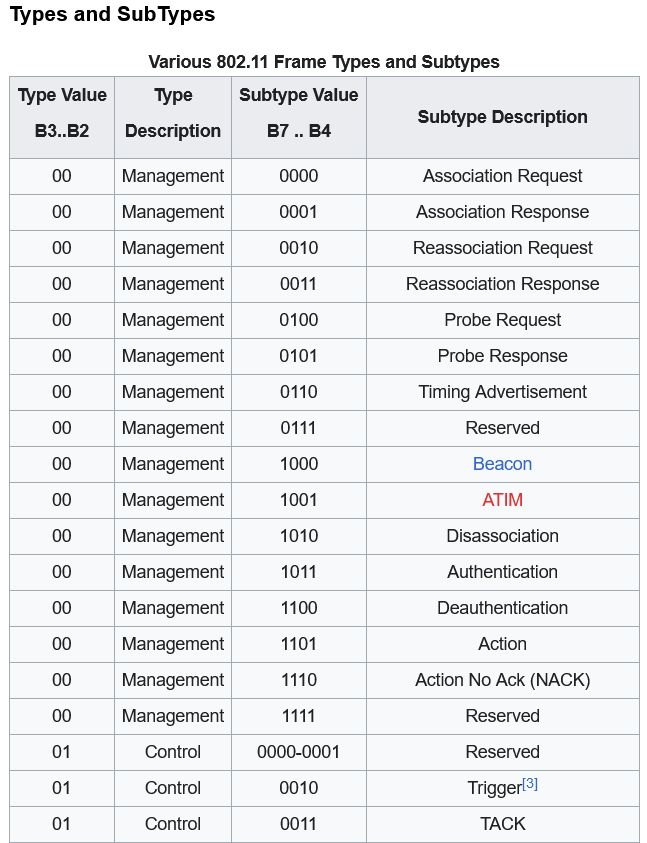
\includegraphics[width=0.5\textwidth]{Latex-Files/Billeder/WIFI_Types.png}
    \caption{WiFi typer og subtyper}
    \label{Wifi Types}
\end{figure}

In 802.11 there are 3 frame types: Management frames, control frames and data frames \cite{Amit802.11frames, DefinitiveGast}. Figure \ref{Wifi Types} shows some of the types and subtypes of different frames with a focus on management frames, since that is what our project is focused on.  Management frames are used by AP's to join and leave the basic service set. They are needed because it is much harder to connect to a specific wireless network rather than a wired network as that is almost automatic when a wire is connected. A wireless network needs to associate a client from a certain sender and ignore others. For clients to know which networks are around them they need to know data about them, this is done via 2 ways of scanning: Active scanning and passive scanning. In passive scanning the client scans every channel passively and listens for beacon frames from AP's, this has the consequence that clients can miss a beacon frame from an AP, since it has to go through every available channel. A beacon frame gives basic information about the AP and are sent continuously by every AP. In active scanning a client sends out probe requests on the channels and listens for probe responses from all the AP's that answer, this has the consequence that a client almost certainly gets information about every single AP in the area. The probe responses gives the client the SSID and capabilities of the AP's. 

Wireless networks also need security while sending packets, i.e. authentication and confidentiality. To ensure confidentiality data frames are encrypted with some sort of security standard. The oldest widespread type being Wired Equivalent Privacy (WEP). It had major security flaws that allows hackers to bypass the algorithm and read the data being sent \cite{WEP1}. Therefore was WiFi Protected Access (WPA) developed in 2003 \cite{WEP3}. 

WEP uses a secret key to encrypt packets between client and AP \cite{WEP2}. The problem with this is that WEP uses the RC4 encryption algorithm, which is known as a stream cipher. A stream cipher operates by making a short key into an infinite random key-stream. The client uses XOR on the key-stream with the plain data to produce the encrypted data. The AP has a copy of the same used key, and uses it to generate an identical key-stream. The AP then uses XOR on the key-stream with the encrypted data to get the exact same plain data back. This type of encryption is easy to misuse, since by flipping a single bit in the encrypted data, the plain data will also have a corresponding single bit flipped. Also the XOR can be found via statistical analysis of key-streams to thereby recover the plain data.

WEP has incorporated defenses against these 2 types of attacks, but they are implemented poorly. The defense against flipping bits are integrity checks in the packet implemented as a CRC-32 checksum. Sadly it is linear which means that it is possible to find the difference between 2 CRC's because the bits that are flipped in the encrypted data is deterministic and therefore an attacker can adjust the checksum and then it is believed that the integrity of the packet is kept, when in reality it isn't.

The defense against the statistical attack is an initialization vector to decrease the chance of reuse of key-streams. The vector is only a 24 bit field and that guarantees the reuse of key-streams. Because of this, the attacker can easily pick up enough data to perform statistical analysis of packets using the same key-stream and then recover the plain data.

WPA2 was a development of the intermediate measure WPA, as a security update to fix many of WEP's problems \cite{WPA2_1}\cite{WEP3}. It was released in 2004 in the 802.11i amendment to the original 802.11. WPA2 uses CCMP protocol which is a development of the AES security algorithm. It rids the network encryption of the previously mentioned security vulnerabilities. 
\\
\begin{figure}[!htbp]
    \centering
    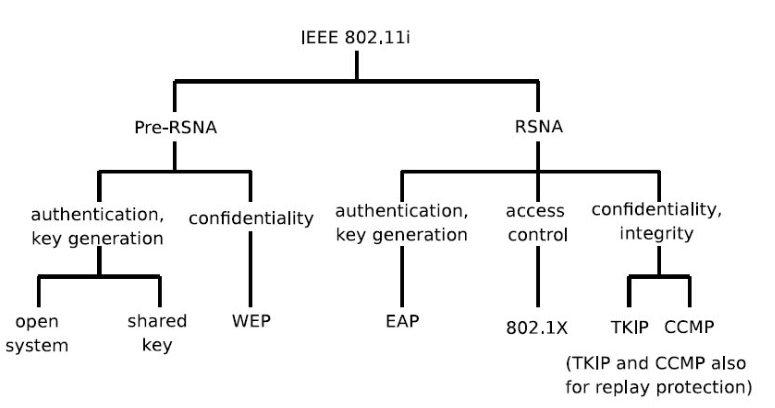
\includegraphics[width=0.6\textwidth]{Latex-Files/Billeder/802.11i security.png}
    \caption{Summary of 802.11i security \cite{WPA2_3}}
    \label{802.11 Security}
\end{figure}

Figure \ref{802.11 Security} shows the different types of securities in the 802.11i standard. It is split up into pre-RSNA and RSNA. Robust
Security Network Association (RSNA) is the way to describe the updated security protocols established with 802.11i and basically means that all security before this standard is out of date. 

For a product to be WiFi certified it requires the usage of a modern security protocol, which is WPA2 \cite{WPA2_2}. New security vulnerabilities have since been found in WPA2 and WPA3 has been created to solve some of those, WPA3 is planned to be implemented widepsread soon. Our focus is not to try decrypting WPA2 or WPA3. 

The authentication of clients and AP's can be exploited by deauthentication attacks. A deauthentication attack is a type of wireless network attack that involves sending forged deauthentication packets to a target client or AP. The theory behind this attack is based on the 802.11 standard, which allows clients to disconnect from an AP using a deauthentication frame.

When a client device is connected to a WiFi network, it sends periodic beacon frames to the access point to maintain the connection. In a deauthentication attack, an attacker sends a series of forged deauthentication packets to the target client or access point, pretending to be the legitimate access point or client. This causes the target to disconnect from the network and require reauthentication, disrupting the communication between the client and the access point.

Deauthentication frames are frames of the management type as seen in figure \ref{Wifi Types}, and have the overall structure as such. Therefore the deauthentication frame contians, among other things, 3 addresses. These three addresses are what can be altered in order to perform a deauthentication attack. One part of the frame body in a deauthentication frame is the reason code, this defines the reason for the termination of the connection. There are 25 different standard reasons defined by Cisco \cite{Cisco_Deathentication_reasoncodes}, these are the ones we will be referring to during the project. Apart from a reasoncode, the frame body includes vendor specific elements, and the Management MIC IE(MMIE) \cite{IEEE_802.11w}. Though this is not always present. The MMIE is only in use when protected management frames are enabled \cite{IEEE_802.11w}. Protected management frames where introduced in order to combat e.g. the deauthentication attack. Since the deauthentication frames are not encrypted in any way, this creates a sizeable vulnerability for a network.

802.11w, realesed in 2009, introduces protected management frames thereby combatting attacks such as deauthentication attacks. This is achieved by ensuring the integrity in the management frame. The integrity check is achieved by the sender calculating a message integriy check(MIC) value, and appending this to the frame. The reciever then calculates the MIC value using the same algorithm, and compares the two. If the two MIC values match, the frame is considered to not having been tampered with, and thus marking it as authentic. Furthermore a frame sequence number(FSN) is introduced, which is used to prevent replay attacks. Replay attacks are not something we will be covering in this project and therefore it wont be analyzed in this report. 

\section{Main Challenges}
Our main challenge in this project is the fact that internet traffic is hard to figure out. There is a lot of data being sent constantly and most of it is not relevant to what we are doing. As we are working with a shared medium it can be hard to differentiate what we are creating and what is part of the standard traffic. Furthermore this makes it difficult to figure out what is going on 'under the hood' when testing our implementations. Thus it has so far taken much longer to perform some of the basic steps of mapping the network and simple deauthentication. Still this is very much a learn by doing project in the way that we obtain solutions to either tackle or overcome the obstacles.

Likewise the theory behind most of the 802.11 management frames and such used in this project is very new to us, since only a short overview of 802.11 has been provided in our courses where the focus mainly has been on the EAPOL 4-way-handshale within WPA. Thus there is a great gap in knowledge we need to fill as some of the implementation parts require a deep understanding of how e.g. the procedure for deauthentication works. 

When we have to decrypt WEP, we have to find some way of getting packets encrypted with WEP, so we either have to find a tool to create WEP packets or find a router that is old enough to be able to create them. 


\section{Time Plan}
In order to generalize and create a overview of our project a timeplan has been created, seen in figure \ref{timeplan}. It is though hard to be sure of what is done when and to give a certain time for each thing. Already now in the process of implementation there has been several obstacles as described in the Main Challenges.  As we are also still early in the process it is still hard to figure out exactly what is needed when and if some of the blocks are even possible to do. 
\\
\begin{figure}[!htbp]
    \centering
    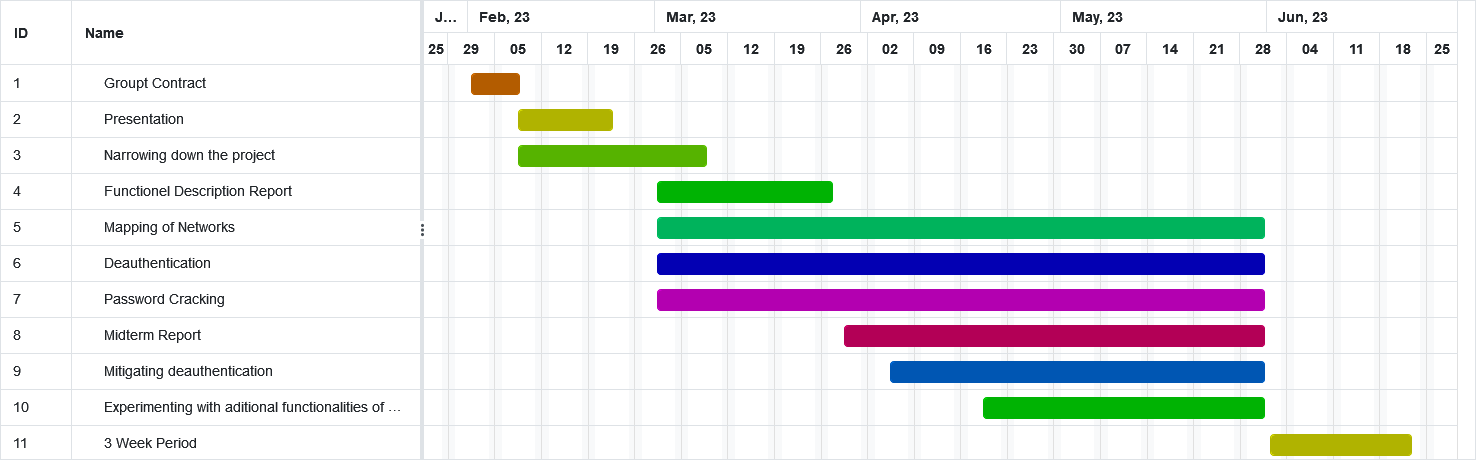
\includegraphics[width=1\textwidth]{Latex-Files/Billeder/Timeplan.png}
    \caption{Timeplan}
    \label{timeplan}
\end{figure}


\section{Conclusion}

We have investigated network traffic via mapping a local WiFi network using Python and the tool scapy to show all AP's connected and sending beacon frames and the clients connected to these networks. We also did deauthentication attacks to disconnect one or more clients from using wireless networking. By doing this we gained advanced knowledge about different types of frames and subframes in the 802.11 standard. We also investigated security in the 802.11 standard, both WEP and WPA2, the 2 most common security algorithms for ensuring the security and integrity of packets and data-streams. Doing this project we also increased our knowledge of python programming and networking toolboxes that use python, which gives a broad understanding of how packets are built in python and in general. 
In the further work on this project, our aim is to gain an even deeper understanding of the processes involved in mapping network, deauthenticating and password cracking. 



%


\newpage
\printbibliography %Prints bibliography
\end{document}
